% MAIN DOC
% Example for dissertation.sty
\documentclass[
  % Replace oneside by twoside if you are printing your thesis on both sides
  % of the paper, leave as is for single sided prints or for viewing on screen.
  % oneside,
  twoside=false,
  fontsize=12pt,% NewsGotT
  paper=a4,
  footinclude=true,
  headinclude=true,
  cleardoublepage=empty,
  headsepline=true,
  headheight=20pt,
  footheight=20pt,
  automark,
  markcase=upper,
  bibliography=totoc,
  %appendix=totoc
  %pagestyle=myheadings
  %footsepline=true,
]{scrbook}

% use the formatting style defined (this file should include all other packages)
%\usepackage{./sty/dissertation}% pdflatex
\usepackage{./sty/dissertation-xelatex}% xelatex

% fixing \vbox and \hbox underfull and overfull
% src: https://tex.stackexchange.com/a/387912
\raggedbottom%

%\addtokomafont{section}{\clearpage}
\addtokomafont{caption}{\small}

%this shall be the last thing in the acronym configuration!!
\makeglossaries%

%% **MORE INFO** %%
%to add the acronyms list add the following where you want to print it:
%\printglossary[type=\acronymtype]
%\clearpage
%\thispagestyle{empty}

%to use an acronym:
%\gls{qps}

% Reverse side notes
% How to generate 2 different files based on conditionals
% https://tex.stackexchange.com/a/220101
% see also makefile rule all-comm
\ifdef{\comm}{\reversemarginpar}

% ------------------------------------------------------------------------
% Title
\mytitle% defined in .sty file

% Glossaries & Acronyms
%\makeglossaries  %  either use this ...
%\makeindex	   % ... or this

% Define Acronyms
%%!TEX root = ../dissertation.tex
%
% here are the acronym entries
\newacronym{mei}{MEI}{Mestrado em Engenharia Inform\'{a}tica}
\newacronym{um}{UM}{Universidade do Minho}
\newacronym{di}{DI}{Departamento de Inform\'{a}tica}
%
\newacronym{qos}{QoS}{Quality of Service}
\newacronym{soa}{SOA}{Service Oriented Architecture}
%
\newacronym{oop}{OOP}{Object Oriented Programming}
\newacronym{oose}{OOSE}{Object Oriented Software Engineering}
\newacronym{omt}{OMT}{Object-Modeling Technique}
\newacronym{vdi}{VDI}{Verein Deutscher Ingenieure}
\newacronym{api}{API}{Application Programming Interface}
\newacronym{pwm}{PWM}{Pulse-Width Modulation}
\newacronym{ic}{IC}{Integrated Circuit}
\newacronym{ssr}{SSR}{Solid-State Relay}
\newacronym{pid}{PID}{Proportional Integrative Derivative}
\newacronym{pci}{PCI}{Peripheral Component Interconnect}
\newacronym{pcb}{PCB}{Printed Circuit Board}
\newacronym{io}{I/O}{Input/Output}
%
% ========================== Article_Mach ========================
\newacronym{am}{AM}{Additive Manufacturing}
\newacronym{lbam}{LBAM}{Laser-based Additive Manufacturing}
\newacronym{fgm}{FGM}{Functionally Graded Material}
\newacronym{mmfgm}{MMFGM}{Multi-Material Functionally Graded Material}
\newacronym{mmam}{MMAM}{Multi-Material Additive Manufacturing}
\newacronym{oom}{OOM}{Object-Oriented Modelling}
\newacronym{uml}{UML}{Unified Modeling Language}
\newacronym{sls}{SLS}{Selective Laser Sintering}
\newacronym{slm}{SLM}{Selective Laser Melting}
\newacronym{mmsls}{MMSLS}{Multi-Material SLS}
\newacronym{mms}{MMS}{Multi-Material Sintering}
\newacronym{doe}{DOE}{Design Of Experiments}
\newacronym{ai}{AI}{Artificial Intelligence}
\newacronym{cad}{CAD}{Computer-Aided Design}
\newacronym{cae}{CAE}{Computer-Aided Engineering}
\newacronym{cam}{CAM}{Computer-Aided Manufacturing}
\newacronym{stl}{STL}{Standard Tessellation Language}
\newacronym{amf}{AMF}{Additive Manufacturing File}
\newacronym{3mf}{3MF}{3D Manufacturing Format}
\newacronym{pov}{POV}{Persistence Of Vision}
\newacronym{dlp}{DLP}{Digital Light Projector}
\newacronym{tin}{TIN}{Triangular Irregular Network}
\newacronym{nc}{NC}{Numerical Control}
\newacronym{cnc}{CNC}{Computer Numerical Control}
\newacronym{svg}{SVG}{Scalable Vector Graphics}
\newacronym{html}{HTML}{Hypertext Markup Language}
\newacronym{xml}{XML}{eXtensible Markup Language}
\newacronym{gui}{GUI}{Graphical User Interface}
\newacronym{astm}{ASTM}{American Society for Testing and Materials}
\newacronym{fdm}{FDM}{Fused Deposition Material}
\newacronym{fff}{FFF}{Fused Filament Fabrication}
\newacronym{lom}{LOM}{Laminated Object Manufacturing}
\newacronym{pbf}{PBF}{Powder Bed Fusion}
\newacronym{ded}{DED}{Direct Energy Deposition}
\newacronym{dld}{DLD}{Direct Laser Deposition}
\newacronym{ebm}{EBM}{Electron Beam Melting}
% ================================================================
%
\newacronym{vm}{VM}{Virtual Machine}
\newacronym{lvm}{LVM}{Linux Virtual Machine}
\newacronym{usb}{USB}{Universal Serial Bus}
\newacronym{cli}{CLI}{Command Line Interface}
\newacronym{rtos}{RTOS}{Real-Time Operating System}
\newacronym{ui}{UI}{User Interface}
%
% Final report
\newacronym{qfd}{QFD}{Quality Function Deployment}
%\glsaddall[types={\acronymtype}]

\begin{document}
	% Cover page ---------------------------------------
%	\umfrontcover%	
	\umtitlepage%
%
%% UNUSED - the title should be modified in \mytitle contained in *.sty file

% Title
\titleA{First Part of Title}
\titleB{Second Part of Title} % (if any)
\subtitleA{First Part of Subtitle}
\subtitleB{Second part of Subtitle} % (if any)

% Author
\author{Author of the Thesis}

% Supervisor(s)
\supervisor{The Supervisor of the thesis}
\cosupervisor{The cosupervisor of the thesis}

% University (uncomment if you need to change default values)
% \def\school{Escola de Engenharia}
% \def\department{Departamento de Inform\'{a}tica}
% \def\university{Universidade do Minho}
% \def\masterdegree{Computer Science}

% Date
\date{\myear} % change to text if date is not today

% Keywords
%\keywords{master thesis}

% Glossaries & Acronyms
%\makeglossaries  %  either use this ...
%\makeindex	   % ... or this

% Define Acronyms
%%!TEX root = ../dissertation.tex
%
% here are the acronym entries
\newacronym{mei}{MEI}{Mestrado em Engenharia Inform\'{a}tica}
\newacronym{um}{UM}{Universidade do Minho}
\newacronym{di}{DI}{Departamento de Inform\'{a}tica}
%
\newacronym{qos}{QoS}{Quality of Service}
\newacronym{soa}{SOA}{Service Oriented Architecture}
%
\newacronym{oop}{OOP}{Object Oriented Programming}
\newacronym{oose}{OOSE}{Object Oriented Software Engineering}
\newacronym{omt}{OMT}{Object-Modeling Technique}
\newacronym{vdi}{VDI}{Verein Deutscher Ingenieure}
\newacronym{api}{API}{Application Programming Interface}
\newacronym{pwm}{PWM}{Pulse-Width Modulation}
\newacronym{ic}{IC}{Integrated Circuit}
\newacronym{ssr}{SSR}{Solid-State Relay}
\newacronym{pid}{PID}{Proportional Integrative Derivative}
\newacronym{pci}{PCI}{Peripheral Component Interconnect}
\newacronym{pcb}{PCB}{Printed Circuit Board}
\newacronym{io}{I/O}{Input/Output}
%
% ========================== Article_Mach ========================
\newacronym{am}{AM}{Additive Manufacturing}
\newacronym{lbam}{LBAM}{Laser-based Additive Manufacturing}
\newacronym{fgm}{FGM}{Functionally Graded Material}
\newacronym{mmfgm}{MMFGM}{Multi-Material Functionally Graded Material}
\newacronym{mmam}{MMAM}{Multi-Material Additive Manufacturing}
\newacronym{oom}{OOM}{Object-Oriented Modelling}
\newacronym{uml}{UML}{Unified Modeling Language}
\newacronym{sls}{SLS}{Selective Laser Sintering}
\newacronym{slm}{SLM}{Selective Laser Melting}
\newacronym{mmsls}{MMSLS}{Multi-Material SLS}
\newacronym{mms}{MMS}{Multi-Material Sintering}
\newacronym{doe}{DOE}{Design Of Experiments}
\newacronym{ai}{AI}{Artificial Intelligence}
\newacronym{cad}{CAD}{Computer-Aided Design}
\newacronym{cae}{CAE}{Computer-Aided Engineering}
\newacronym{cam}{CAM}{Computer-Aided Manufacturing}
\newacronym{stl}{STL}{Standard Tessellation Language}
\newacronym{amf}{AMF}{Additive Manufacturing File}
\newacronym{3mf}{3MF}{3D Manufacturing Format}
\newacronym{pov}{POV}{Persistence Of Vision}
\newacronym{dlp}{DLP}{Digital Light Projector}
\newacronym{tin}{TIN}{Triangular Irregular Network}
\newacronym{nc}{NC}{Numerical Control}
\newacronym{cnc}{CNC}{Computer Numerical Control}
\newacronym{svg}{SVG}{Scalable Vector Graphics}
\newacronym{html}{HTML}{Hypertext Markup Language}
\newacronym{xml}{XML}{eXtensible Markup Language}
\newacronym{gui}{GUI}{Graphical User Interface}
\newacronym{astm}{ASTM}{American Society for Testing and Materials}
\newacronym{fdm}{FDM}{Fused Deposition Material}
\newacronym{fff}{FFF}{Fused Filament Fabrication}
\newacronym{lom}{LOM}{Laminated Object Manufacturing}
\newacronym{pbf}{PBF}{Powder Bed Fusion}
\newacronym{ded}{DED}{Direct Energy Deposition}
\newacronym{dld}{DLD}{Direct Laser Deposition}
\newacronym{ebm}{EBM}{Electron Beam Melting}
% ================================================================
%
\newacronym{vm}{VM}{Virtual Machine}
\newacronym{lvm}{LVM}{Linux Virtual Machine}
\newacronym{usb}{USB}{Universal Serial Bus}
\newacronym{cli}{CLI}{Command Line Interface}
\newacronym{rtos}{RTOS}{Real-Time Operating System}
\newacronym{ui}{UI}{User Interface}
%
% Final report
\newacronym{qfd}{QFD}{Quality Function Deployment}
%\glsaddall[types={\acronymtype}]



\ummetadata % add metadata to the document (author, publisher, ...)

%\maketitle % should use a customized title creation
% see: https://en.wikibooks.org/wiki/LaTeX/Title_Creation
  % Add dedication
%  %\chapter*{Dedication}
% src: https://tex.stackexchange.com/a/167529
% see also: .sty file (lines 297-309)
\begin{dedicat}
  %\usefont{T1}{LobsterTwo-LF}{bx}{it}
  % src: https://en.wikibooks.org/wiki/LaTeX/Fonts
  \rmfamily
  {\Large To my parents,}\\
  {\large for always pushing me forward.}
  \par   %% or a blank line
  \vspace{4\baselineskip}
  
  \normalfont
  \emph{"Wir m{\"u}ssen wissen,\\ 
  Wir werden wissen"}\\
  \vspace{\baselineskip}
  David Hilbert, 1930

\end{dedicat}

%%
%% ----------License------
%  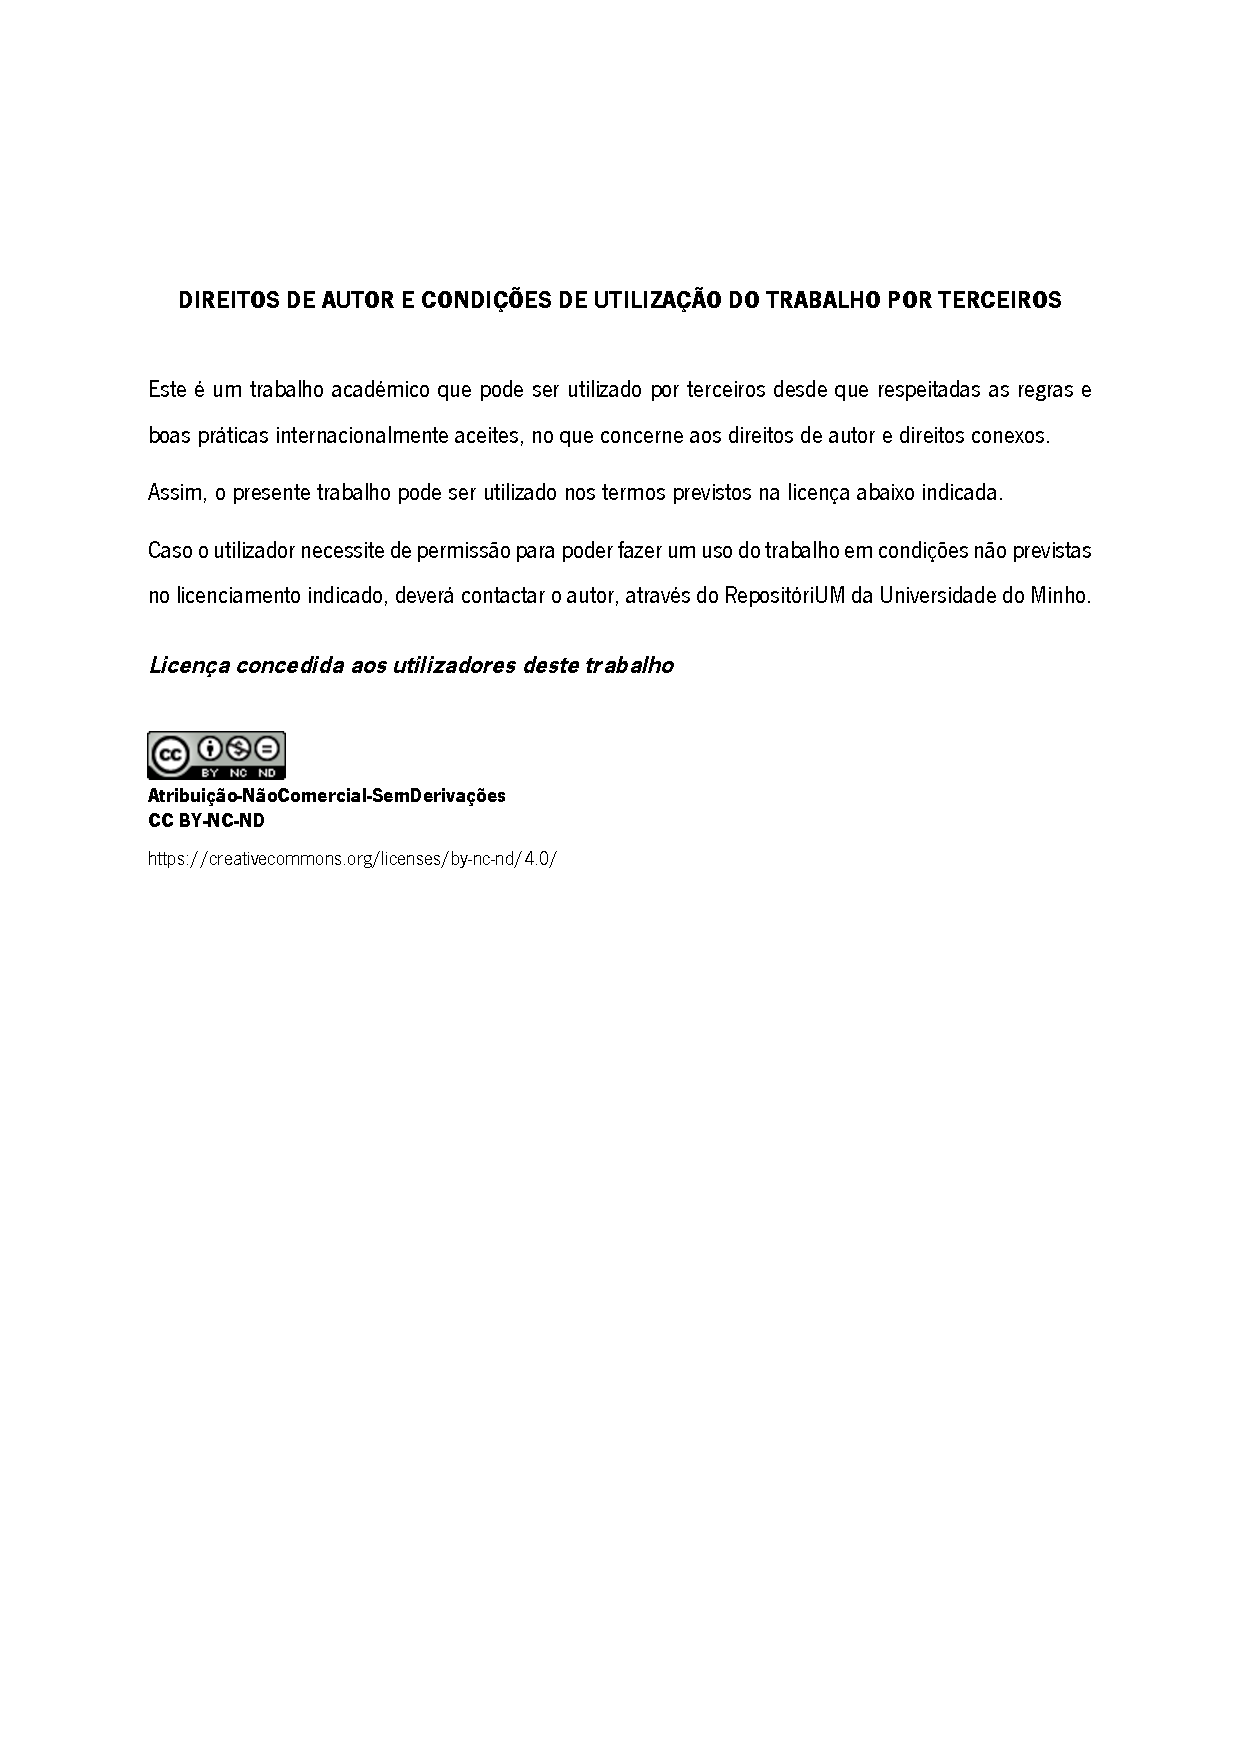
\includepdf[pages=-]{anexo3-license}
%  \cleardoublepage%
%%---------------------
%	% Add acknowledgements ----------------------------
%  \chapter*{Acknowledgements}
First and foremost, I would like to thank...
%%% Local Variables:
%%% mode: latex
%%% TeX-master: "../../dissertation"
%%% End:

%  %\chapter*{Acknowledgements}
%  %	Write acknowledgements here
%  \cleardoublepage%
%%---------------------
%  %
%  \KOMAoption{fontsize}{11.5pt}%
%	% Add abstracts (en,pt) ---------------------------
%  \chapter*{Abstract}
Functional design is the desirable and most sustainable method to design
products: by adding the material only where is strictly required to perform its
function, the resources usage is optimized, especially materials and
energy. However, functional design may dictate the usage of several materials or a combination of them to fulfill its goal, which is hindered by the
current manufacturing methodologies. An example of a class of
products where functional design is key is biomedical implants, like the hip implant.

% Keywords
\keywords{functional design, multimaterial, laser based additive manufacturing}
%%% Local Variables:
%%% mode: latex
%%% TeX-master: "../../dissertation"
%%% End:

%  %\chapter*{Abstract}
%	%Write abstract here (en) or import corresponding file	
%  \cleardoublepage%
%%
%  \KOMAoption{fontsize}{11pt}%
%  \chapter*{Resumo}
\selectlanguage{portuguese}%
O design funcional é o método mais desejável e sustentável de projetar
produtos: adicionando material somente é estritamente necessário para
a sua função, o uso de recursos é otimizado, especialmente materiais e

\keywordspt{design funcional, multimaterial, manufatura aditiva baseada em laser}
\selectlanguage{english}%
%%% Local Variables:
%%% mode: latex
%%% TeX-master: "../../dissertation"
%%% End:

%  %\chapter*{Resumo}
%	%Escrever aqui resumo (pt), ou importar respectivo ficheiro,
%  \cleardoublepage%
	% Summary Lists ------------------------------------
  % add toc and lists to TOC
  % src: https://tex.stackexchange.com/a/74440
%  \KOMAoption{fontsize}{12pt}%
  % TOC
  \phantomsection%
  \addcontentsline{toc}{chapter}{Contents}
  \tableofcontents%
  \cleardoublepage%
  % List of Figs
  \phantomsection%
  \addcontentsline{toc}{chapter}{List of Figures}
  \listoffigures%
  \cleardoublepage%
  % List of Tables
  \phantomsection%
  \addcontentsline{toc}{chapter}{List of Tables}
  \listoftables
  \cleardoublepage%
  % List of listings
  \phantomsection%
  \addcontentsline{toc}{chapter}{List of Listings}
  \lstlistoflistings%
  \cleardoublepage%
  % list of Acronyms
  \phantomsection%
  \addcontentsline{toc}{chapter}{List of Abbreviations}
  \listofacronyms%
  \cleardoublepage%
    %\printglossary[type=\acronymtype]%
    %\printglossary[type=\acronymtype]%
 %   \listofabbreviations%
  % List of symbols
  \phantomsection%
  \addcontentsline{toc}{chapter}{List of Symbols}
  \listofsymbols%
  \cleardoublepage%
%
	\thispagestyle{empty}
  %\newpage
	\pagenumbering{arabic}
  %\newpage
  %\setcounter{page}{0}
  %\pagenumbering{arabic}
  %\setcounter{page}{1}
 % 
  % making chapter pages with no header and footer
  \renewcommand*{\chapterpagestyle}{empty}
  %-------------- MAIN BODY CHAPTERS----------------------------------
  % Include the other files (\include adds a blank page between files)
  % - does not need the file extension
%  \KOMAoption{fontsize}{12pt}%
  \setlength{\unitlength}{1mm}
  %% 1,5 line spacing
  \renewcommand{\baselinestretch}{1.5}
%
  % !TEX root = ../dissertation.tex

% For VIM to recognize the document syntax \begin{document} and \end{document}
% - However, the compilation will fail!! So don't forget to comment the
%   directives before compiling!!'

%\begin{document}

% CHAPTER - Introduction -------------------------
\chapter{Introduction}

% To correctly add a marginpar, \mbox needs to be added and a blank line is also
% needed
\ifdef{\comm}{\mbox{}\marginpar{Intro}}

One of the ultimate goals of engineering is the ability to provide sustained 
development, by efficiently using the available resources --- materials, energy,
knowledge, time. This is a ``Sisyphus's stone''\footnote{King of Ephyra,
condemned to push a stone uphill for eternity --- immortalised in ``The Myth of
Sisyphus'' by Albert Camus}, a perpetual quest for optimisation of efforts and
resources. One such example in the engineering field is the ability to produce
components with the minimum amount of material needed for its function, i.e.,
functional design of components without restrictions to geometry or type and
number of different materials; instead the focus should be on the desired
properties of such components, customising them for the specific field of
application. 

%\begin{document}
\section{Context}
The functional design of components is a complex topic, with a myriad of
questions to be answered: what is the function of the component?; what design
criteria must be met to fulfil its function?; how will the component be
produced, and what data does it require?; how will the component's performance
be measured?, among others. The answers are often not clear or simple as they
dictate the use of several materials and several manufacturing technologies,
increasing severely the complexity of producing such components: how to
effectively combine two or more materials into a single component in a
synergistic way?

%%% Local Variables:
%%% mode: latex
%%% TeX-master: "../../../dissertation"
%%% End:

%\begin{document}
\section{Motivation and Goals}
The main goal of this project is to develop a remote controlled vehicle with the
following characteristics:
\begin{enumerate}
  \item Remotely operated: the vehicle must be remotely operated to enable its
    usage in critical or unaccessible areas to human operators;
  \item Provide visual feedback to the user: to be a valuable asset in the
    exploration and maintenance domains, the vehicle must provide visual
    feedback to the user of its surroundings.
  \item Safe: the vehicle must be safe to use and prevent its damage and of its
    surroundings
  \item Robust: the vehicle must be able to sustain harsh environmental
    conditions and provide redundant mechanisms to avoid control loss.
  \item Affordable: so it can be an economically viable product.
  \end{enumerate}
%%% Local Variables:
%%% mode: latex
%%% TeX-master: "../../../dissertation"
%%% End:

%\begin{document}
\section{Main objectives}
The goal of the present work is to close the gap between design and fabrication of
multi-material components from metallic/ceramic materials using
\gls{sls}/\gls{slm} technology. To this end several main objectives have been
outlined:
\begin{enumerate}
  \item Develop a design methodology for multi-material fabrication of
    metals/ceramics;
  \item Instantiate a practical workflow and respective toolchain from the
    design methodology;
  \item Develop and build a proof-of-concept equipment capable of producing
    such components;
  \item Test the production of multi-material components using the proposed
    workflow/toolchain and the equipment built.
  \end{enumerate}

  This is \gls{pi}
  
  This is \gls{omega}
%%% Local Variables:
%%% mode: latex
%%% TeX-master: "../../../dissertation"
%%% End:

%
\section{Research hypothesis (optional)}

  Reseach hypothesis


%\begin{document}
\section{Thesis organisation}
This thesis is organised as follows:
In Chapter~\ref{ch:state-art}, the state of the art of the additive
manufacturing technology, \gls{lbam}, and \gls{mmam} is presented, with special
focus on the last, namely on \gls{fgm} structures. Lastly, a brief overview of
the available methodologies in these fields are presented.

In Chapter~\ref{ch:theor-found} the theoretical foundations are presented, namely the project development methodologies and associated tools,
and the \gls{sls}/\gls{slm} process in detail.

In Chapter~\ref{ch:prob-challenge}, the multi-material design and production
problem and its challenges using \gls{sls}/\gls{slm} technology are
presented. The methodology devised for multi-material production through the
\gls{lbam} technology is presented to tackle the high complexity of the process
and the lack of a supporting methodology, taking into account the key agents of
the process and leveraging the process information.

In Chapter~\ref{ch:development} is presented all the development phase of the
project. A specific workflow was instantiated from
the methodology, attending to the specific requirements and constraints of the
project. Based on this workflow, a toolchain was assembled, designing the
required software components. Finally, based on the requirements and constraints
of the process itself, the mechanical and electronic infrastructures were
designed, and on top of the last, the control software was designed.

In Chapter~\ref{ch:application}, the workflow and equipment were put to the test
to verify their suitability to the process and their performance for
multi-material component production. Additionally, production manufacturing tests
were also performed. Tests were used to validate the workflow and equipment,
pointing out also straightforward ways to adapt and implement custom paths for
the multi-material \gls{lbam} process.

The Chapter~\ref{ch:conclusion} gives a summary of this thesis as well as
prospect for future work.

Lastly, the appendices (see Section~\ref{ch:Append}) contain detailed information...
%%% Local Variables:
%%% mode: latex
%%% TeX-master: "../../../dissertation"
%%% End:


%%% Local Variables:
%%% mode: latex
%%% TeX-master: "../../../dissertation"
%%% End:

  \setcounter{table}{0}
  \setcounter{figure}{0}
%
%  %\begin{document}
	% CHAPTER - State of the Art ---------------------
\chapter{State of the art}
\label{ch:state-art}
In this chapter a review on the state of the art is presented. %
Additive manufacturing is discussed briefly as a preliminary topic. %
Then, Laser-based additive manufacturing processes are discussed as viable
solutions for metallic and composite manufacturing. %

%%% Local Variables:
%%% mode: latex
%%% TeX-master: "../../../dissertation"
%%% End:

%  \setcounter{table}{0}
%  \setcounter{figure}{0}
  %
  % CHAPTER - Theoretical foundations ---------------
\chapter{Theoretical foundations}%
\label{ch:theor-found}
In this chapter some background is provided for the main subjects. The
fundamental technical concepts are presented as they proved its usefulness along
the project, namely the project development methodologies and associated tools,
and communications in detail.
%
%\section{Project methodologies}
\section{Project methodologies}
The methodologies used for the project development are briefly described next.
\subsection{Development methodology of mechatronics --- VDI 2206}
\label{subsec:vdi-2206}

Mechatronics, was defined by Harashima et. al~\cite{harashima1996mechatronics}
as: \emph{''the synergistic integration of mechanical engineering
with electronic and intelligent computer control in the design of industrial
products and processes''}. This definition has more than twenty years, and
nowadays it could be extended to other domains beyond the industrial sector,
but a central idea remains: the synergy between these fields of knowledge, able
% src:
% https://en.wikibooks.org/wiki/LaTeX/Floats,_Figures_and_Captions#Subfloats
\begin{figure}[!hbt]
    \centering
    %\captionsetup[sub]{margin=10pt}
    % a)
    \subcaptionbox{One macro cycle
\label{fig:v-model-macro}}
    [0.5\linewidth]{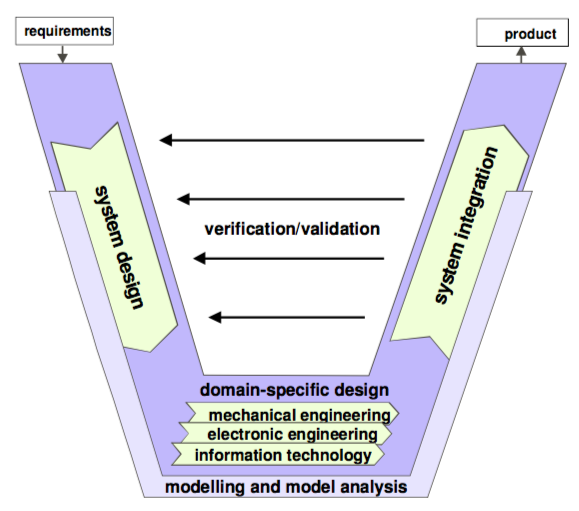
\includegraphics[width=0.45\textwidth]{./img/v-model-macro.png}}
    % b)
    %\subcaptionbox{One macro cycle (refined)~\cite{isermann2008mechatronic} 
    %\label{fig:v-model-isermann}}
    %[0.8\linewidth]{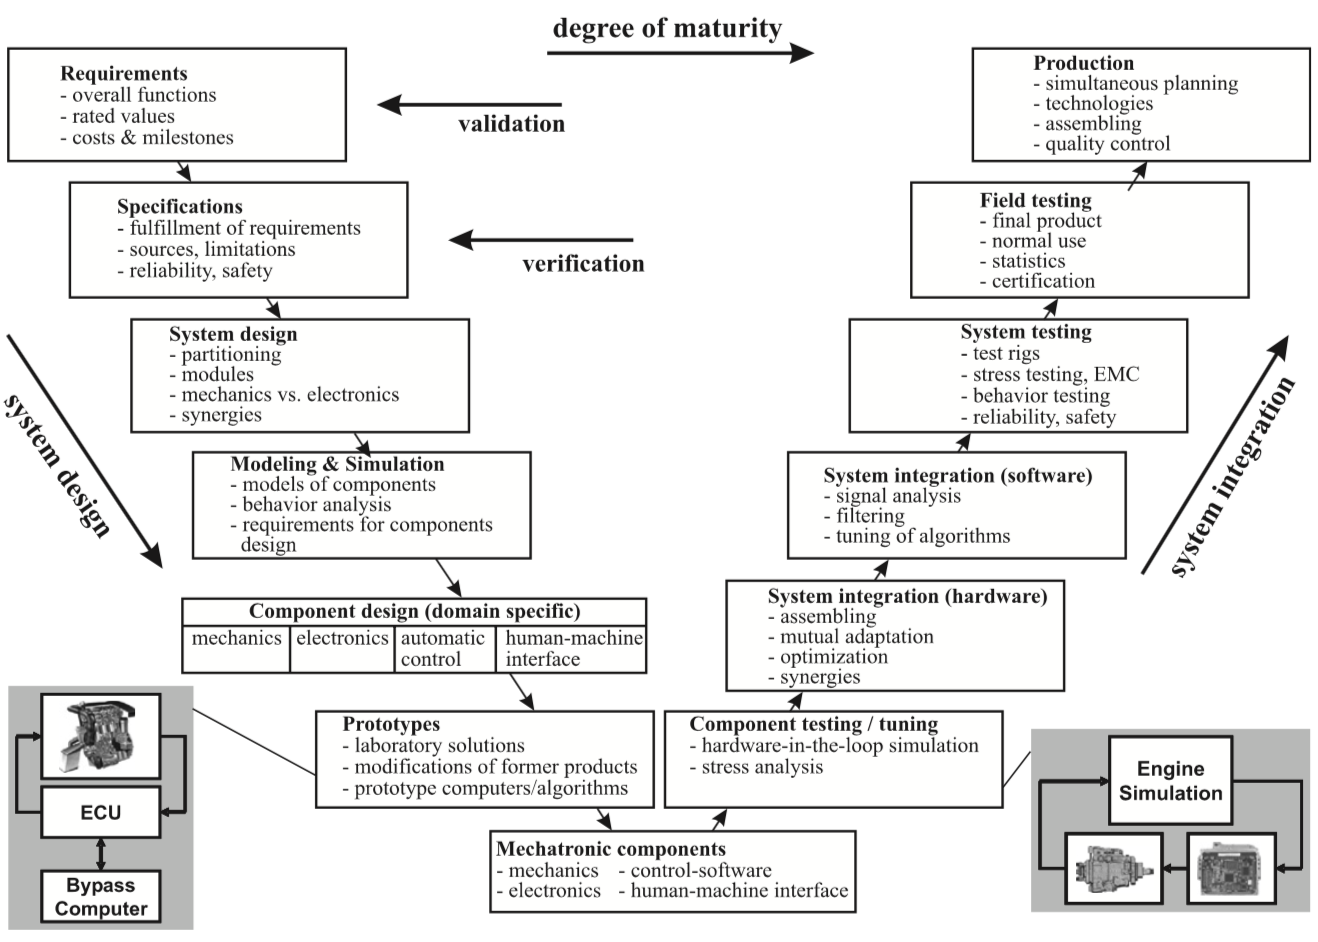
\includegraphics[width=0.8\textwidth]{./img/v-model-isermann.png}}
    % b)
    \subcaptionbox{Iterating over a number of macro-cycles with increasing
      process maturity
\label{fig:v-model-iter}}
    [1.0\linewidth]{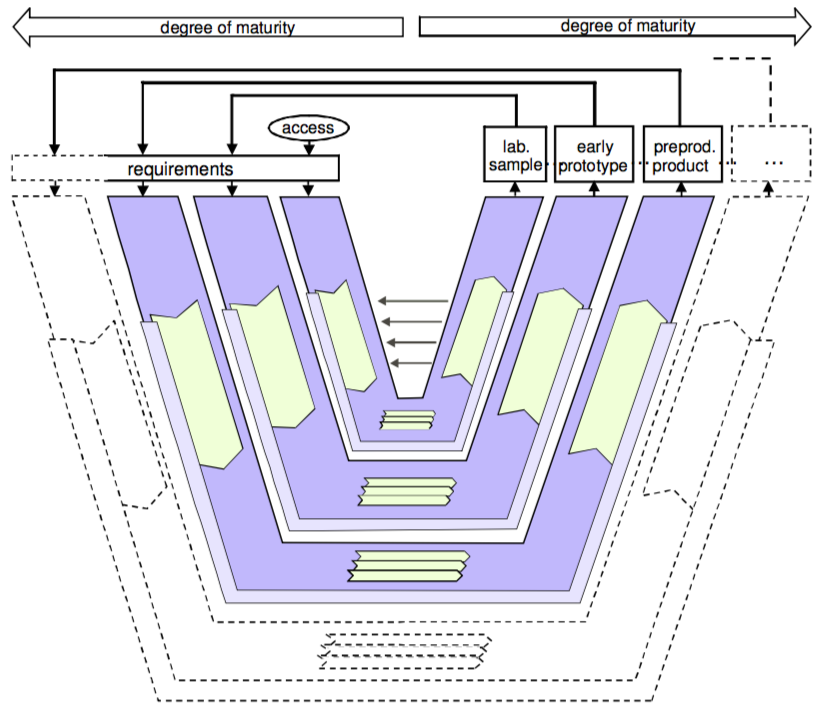
\includegraphics[width=0.55\textwidth]{./img/v-model-iter.png}}
    % c)
    % fig
    \caption{Mechatronics design V-model, VDI 2206 2003~\cite{gausemeier2003new}}
\label{fig:v-model}
\end{figure}

\subsubsection{Process modules for recurrent working steps}
The main phases in the v-model are not yet detailed: this needs to be done by
the designer. However, some design procedures occur regularly during the design
and were identified by field practitioners in terms of predefined process
modules, representing procedures and methods for different design tasks,
organised in a data base
(fig.~\ref{fig:v-model-recurrent}\cite{gausemeier2003new}). The VDI 2206
guideline provides detailed process modules for the V-model macro cycle. One
such example is given in fig.~\ref{fig:v-model-recurrent} for the system design,
which can be described phase-milestone-diagrams, checklists, process-flow
diagrams, etc..

\begin{figure}[!hbt]
  \begin{center}
    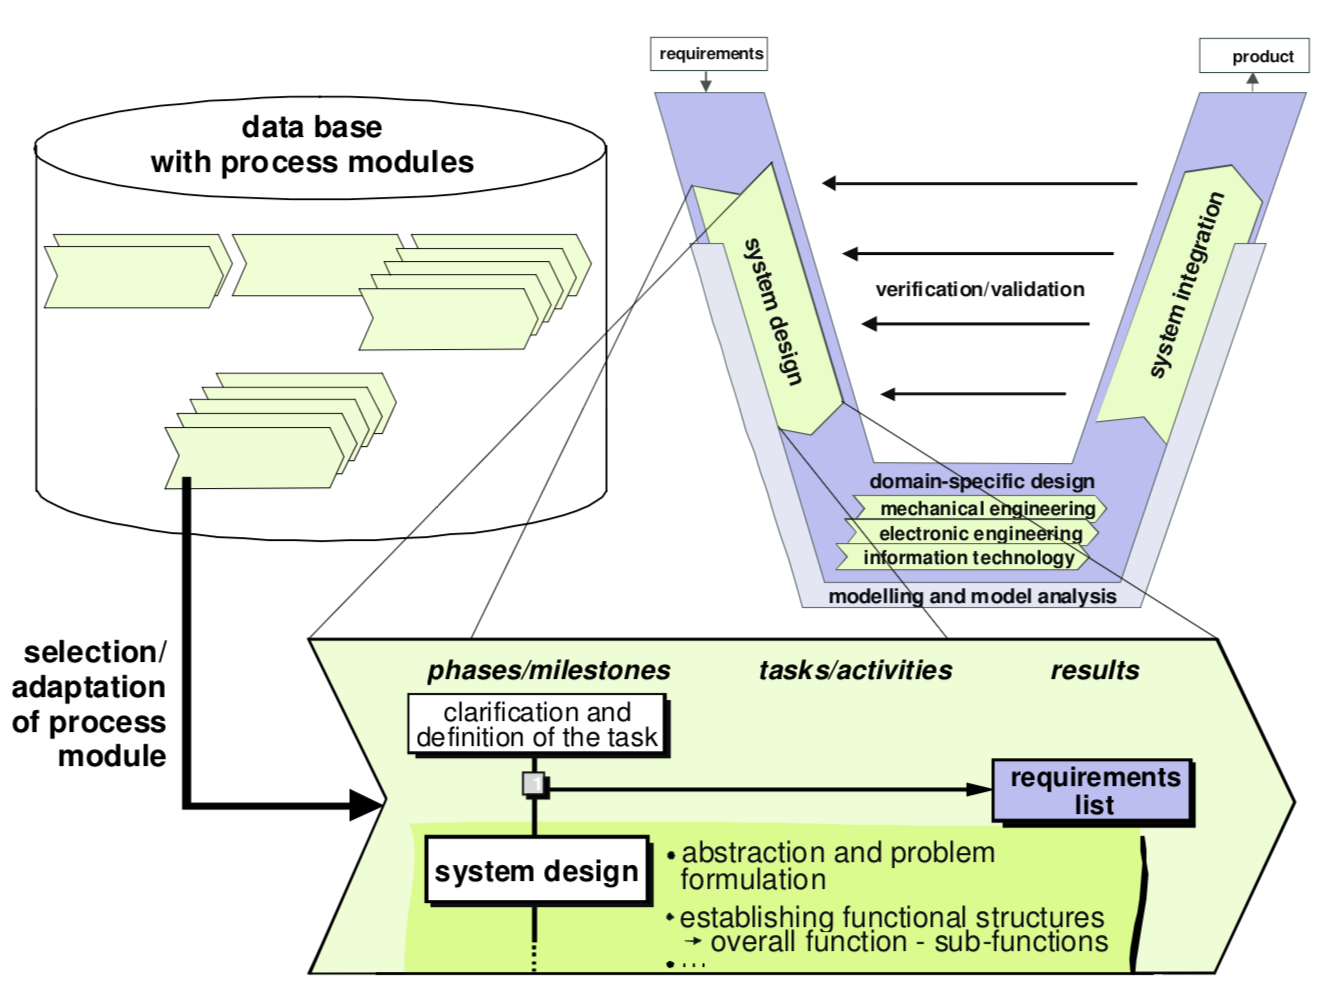
\includegraphics[width=0.65\textwidth]{./img/v-model-recurrent.png}
  \end{center}
  \caption{Configuration of process modules for individual operation steps}
\label{fig:v-model-recurrent}
\end{figure}

%%% Local Variables:
%%% mode: latex
%%% TeX-master: "../../../dissertation"
%%% End:

\subsection{Waterfall}
\label{subsec:waterfall}
For the domain-specific design of software the waterfall methodology is used.
The waterfall model (fig.~\ref{fig:waterfall}) represents the first effort to
conveniently tackle the increasing complexity in the software development
process, being credited to Royce, in 1970, the first formal description of the
model, even though he did not coin the term~\cite{sommerville1996software}. It
envisions the optimal method
as a linear sequence of phases, starting from requirement elicitation to system
testing and product shipment~\cite{cusumano1995beyond} with the process flowing
from the top to the bottom, like a cascading waterfall.

In general, the phase sequence is as follows: analysis, design, implementation,
verification and maintenance.
\begin{enumerate}
  \item Firstly, the project requirements are elicited, identifying the key
    requirements and constraints the system being developed must meet from the
    end-user perspective, captured in natural language in a product requirements document.
  \item In the analysis phase, the developer should convert the application
    level knowledge, enlisted as requirements, to the solution domain knowledge
    resulting in analysis models, schema and business rules.
  \item In the design phase, a thorough specification is written allowing the
    transition to the implementation phase, yielding the decomposition in
    subsystems and the software architecture of the system. 
  \item In the implementation stage, the system is developed, following the
    specification, resulting in the source code.
  \item Next, after system assembly and integration, a verification phase occurs
    and system tests are performed, with the systematic discovery and debugging
    of defects.
  \item Lastly, the system becomes a product and, after deployment, the
    maintenance phase start, during the product life time.
\end{enumerate}
While this cycle occurs, several transitions between multiple phases might
happen, since an incomplete specification or new knowledge about the system,
might result in the need to rethink the document.

The advantages of the waterfall model are: it is simple and easy to understand
and use and the phases do not overlap; they are completed sequentially. However,
it presents some drawbacks namely: difficulty to tackle change and high
complexity and the high amounts of risk and uncertainty. However, in the present
work, due to its simplicity, the waterfall model proves its usefulness and will
be used along the project.

As a reference in the sequence of phases and the expected outcomes from each
one, it will be used the chain of development activities and their products
depicted in fig.~\ref{fig:sw-devel-activities} (withdrawn from
\cite{bruegge2004object}).

\begin{figure}[!hbt]
\centering
    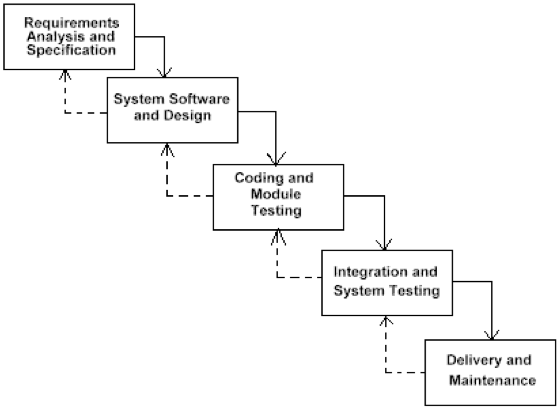
\includegraphics[width=0.6\textwidth]{./img/waterfall.png}
  \caption{Waterfall model diagram}\label{fig:waterfall}
\end{figure}

\subsection{Unified Modeling Language (UML)}
\label{subsec:uml}
To aid the software development process, a notation is required, to articulate
complex ideas succinctly and precisely. The notation chosen was the \gls{uml},
as it provides a spectrum of notations for representing different aspects of a
system and has been accepted as a standard notation in the software
industry~\cite{bruegge2004object}.

The goal of UML is to provide a standard notation that can be used by all
object- oriented methods and to select and integrate the best elements of
precursor software notations, namely \gls{omt}, Booch, and \gls{oose}
~\cite{bruegge2004object}. It provides
constructs for a broad range of systems and activities (e.g., distributed
systems, analysis, system design, deployment). System development focuses on
three different models of the system
(fig.~\ref{fig:sw-devel-activities})~\cite{bruegge2004object}:
\begin{enumerate}
  \item \textbf{\emph{The functional model}}: represented in UML with use case
    diagrams, describes the functionality of the system from the user's point of
    view.
  \item \textbf{\emph{The object model}}: represented in UML with class
    diagrams, describes the structure of the system in terms of objects,
    attributes, associations, and operations.  
  \item \textbf{\emph{The dynamic model}}: represented in UML with interaction
    diagrams, state-machine diagrams, and activity diagrams, describes the
    internal behaviour of the system.
\end{enumerate}

\begin{figure}[!hbt]
\centering
    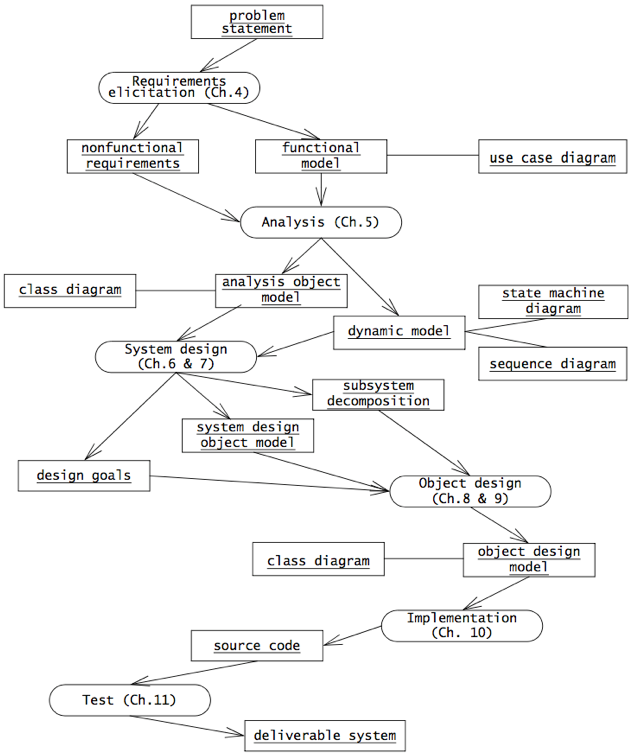
\includegraphics[width=0.7\textwidth]{./img/sw-devel-activities.png}
  \caption{An overview of the object-oriented software engineering development
  and their products. This diagram depicts only logical dependencies among work
  products (withdrawn from~\cite{bruegge2004object})}
\label{fig:sw-devel-activities}
\end{figure}
%%% Local Variables:
%%% mode: latex
%%% TeX-master: "../../../dissertation"
%%% End:

%%% Local Variables:
%%% mode: latex
%%% TeX-master: "../../../dissertation"
%%% End:

%\section{Communications}
% Section: Communications - Handles all communications required for the proj
\section{Communications}
The methodologies used for the project development are briefly described next.
% \subsection{Development methodology of mechatronics --- VDI 2206}
\label{subsec:vdi-2206}

Mechatronics, was defined by Harashima et. al~\cite{harashima1996mechatronics}
as: \emph{''the synergistic integration of mechanical engineering
with electronic and intelligent computer control in the design of industrial
products and processes''}. This definition has more than twenty years, and
nowadays it could be extended to other domains beyond the industrial sector,
but a central idea remains: the synergy between these fields of knowledge, able
% src:
% https://en.wikibooks.org/wiki/LaTeX/Floats,_Figures_and_Captions#Subfloats
\begin{figure}[!hbt]
    \centering
    %\captionsetup[sub]{margin=10pt}
    % a)
    \subcaptionbox{One macro cycle
\label{fig:v-model-macro}}
    [0.5\linewidth]{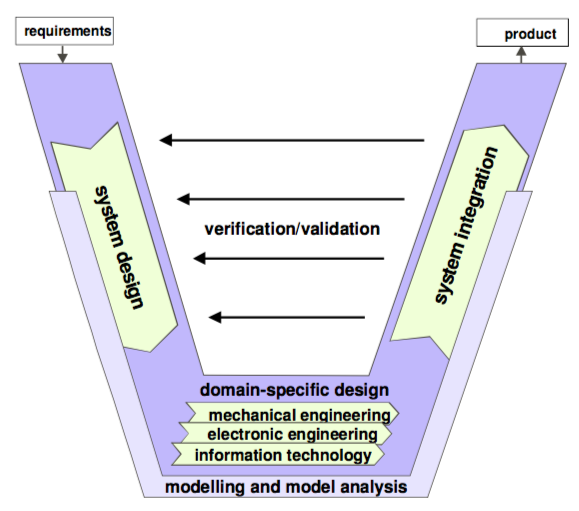
\includegraphics[width=0.45\textwidth]{./img/v-model-macro.png}}
    % b)
    %\subcaptionbox{One macro cycle (refined)~\cite{isermann2008mechatronic} 
    %\label{fig:v-model-isermann}}
    %[0.8\linewidth]{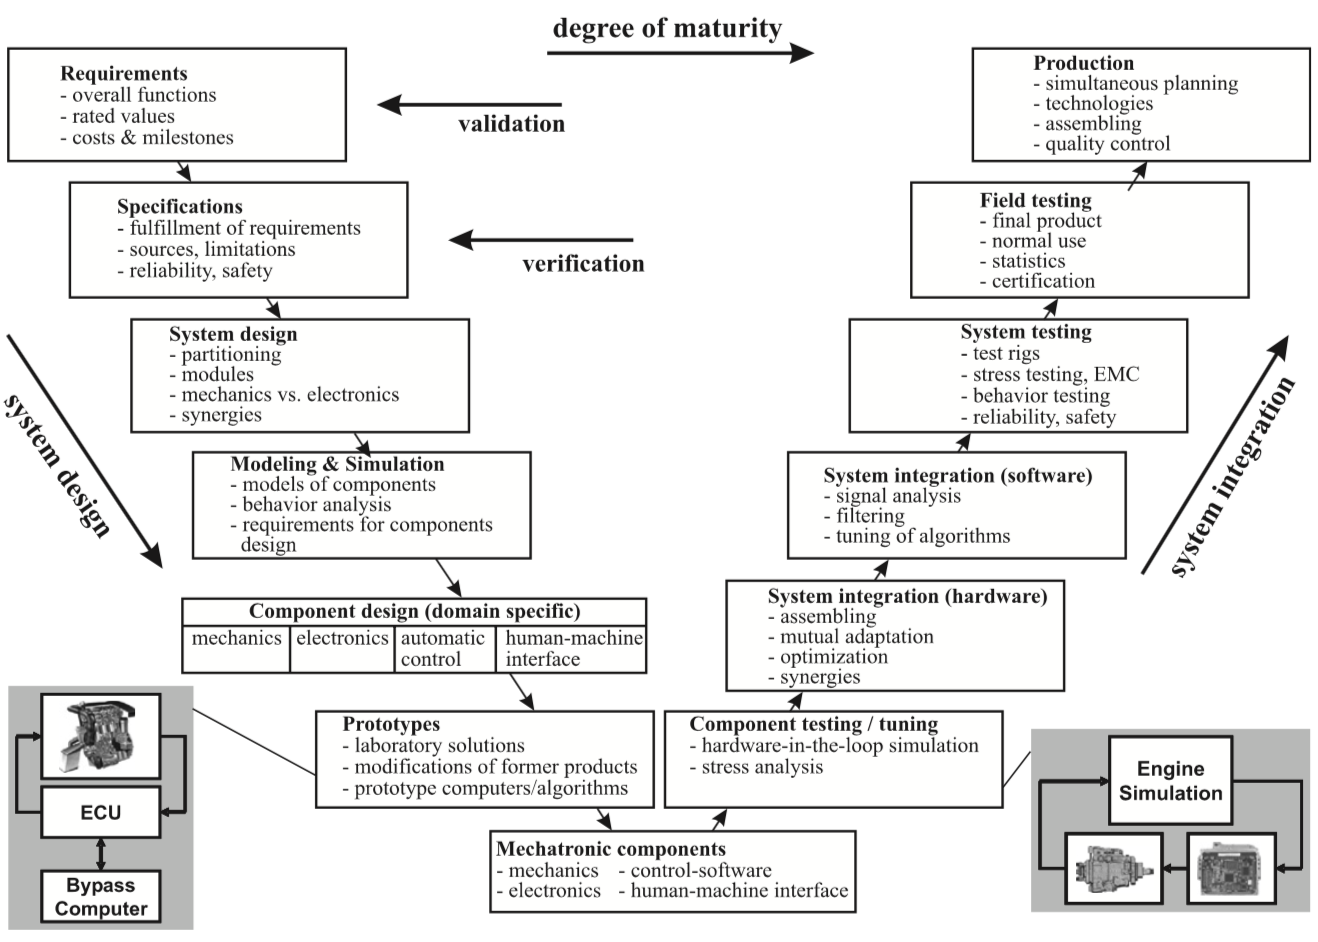
\includegraphics[width=0.8\textwidth]{./img/v-model-isermann.png}}
    % b)
    \subcaptionbox{Iterating over a number of macro-cycles with increasing
      process maturity
\label{fig:v-model-iter}}
    [1.0\linewidth]{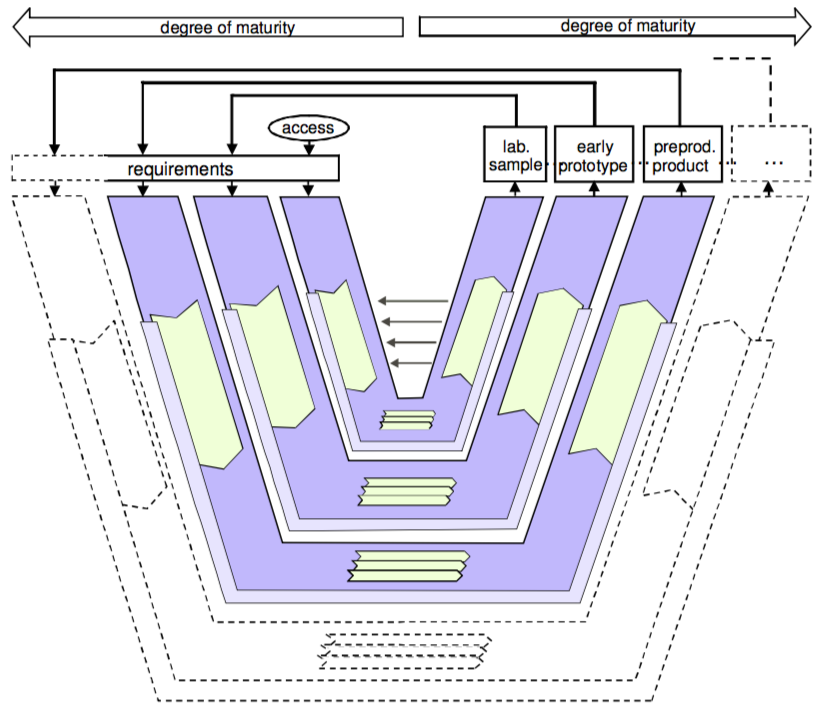
\includegraphics[width=0.55\textwidth]{./img/v-model-iter.png}}
    % c)
    % fig
    \caption{Mechatronics design V-model, VDI 2206 2003~\cite{gausemeier2003new}}
\label{fig:v-model}
\end{figure}

\subsubsection{Process modules for recurrent working steps}
The main phases in the v-model are not yet detailed: this needs to be done by
the designer. However, some design procedures occur regularly during the design
and were identified by field practitioners in terms of predefined process
modules, representing procedures and methods for different design tasks,
organised in a data base
(fig.~\ref{fig:v-model-recurrent}\cite{gausemeier2003new}). The VDI 2206
guideline provides detailed process modules for the V-model macro cycle. One
such example is given in fig.~\ref{fig:v-model-recurrent} for the system design,
which can be described phase-milestone-diagrams, checklists, process-flow
diagrams, etc..

\begin{figure}[!hbt]
  \begin{center}
    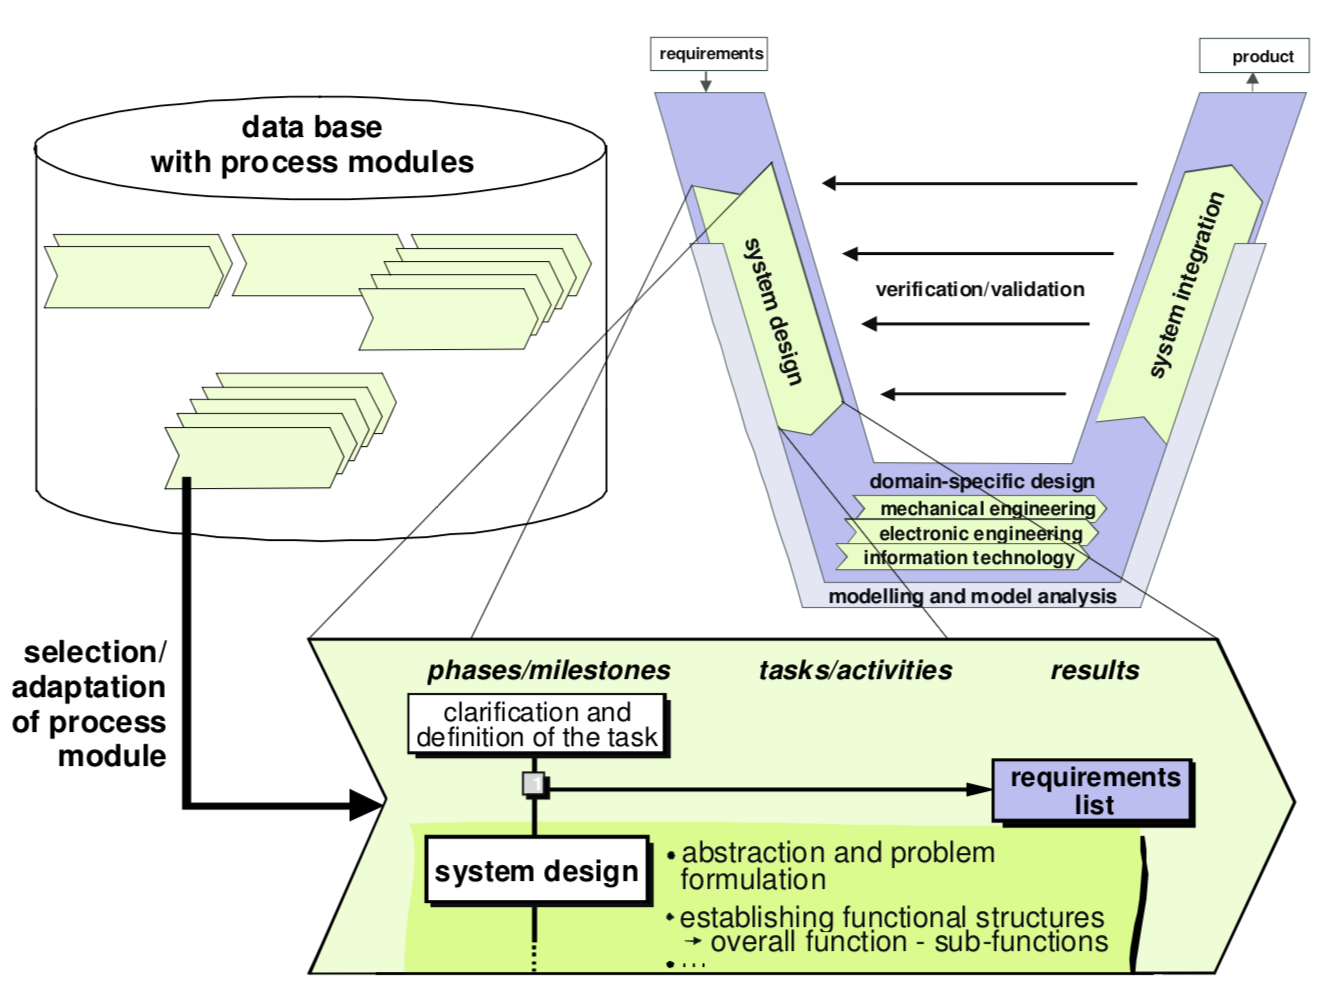
\includegraphics[width=0.65\textwidth]{./img/v-model-recurrent.png}
  \end{center}
  \caption{Configuration of process modules for individual operation steps}
\label{fig:v-model-recurrent}
\end{figure}

%%% Local Variables:
%%% mode: latex
%%% TeX-master: "../../../dissertation"
%%% End:

%
\subsection{Bluetooth}%
\label{sec:bluetooth}
%
\subsubsection{Selecting a target device}%
\label{sec:bt-target-device}
%
\subsubsection{Transport protocols}%
\label{sec:bt-transport-protocols}
%
\subsubsection{Port Numbers}%
\label{sec:bt-port-nrs}
%
\subsubsection{Service discovery}%
\label{sec:bt-service-discovery}
%
\subsubsection{Host Controller Interface --- HCI}%
\label{sec:bt-hci}
%
\subsubsection{Stacks Bluetooth}%
\label{sec:bt-hci}
%
\subsection{GPRS}%
\label{sec:gprs}
%
\subsection{Network programming --- sockets}%
\label{sec:netw-progr-sock}
%
\subsection{Client---server architecture}%
\label{sec:client-serv-arch}
%%% Local Variables:
%%% mode: latex
%%% TeX-master: "../../../dissertation"
%%% End:
%%% Local Variables:
%%% mode: latex
%%% TeX-master: "../../../dissertation"
%%% End:

%\section{Concurrency}
%\label{sec:concurrency}
%      % Concurrency
\section{Concurrency}%
\label{sec:concurrency}
Concurrency is used to refer to things that appear to happen at the same time,
but which may occur serially~\cite{buttlar1996pthreads}, like the case of a multithreaded execution in
a single processor system.
Two concurrent tasks may start, execute and finish in overlapping instants of
time, without the two being executed at the same time.
As defined in POSIX, a concurrent execution requires that a function that
suspends the calling thread shall not suspend other threads, indefinitely.

This concept is different from parallelism. Parallelism refers to the
simultaneous execution of tasks, like the one of a multithreaded program in a
multiprocessor system.
Two parallel tasks are executed at the same time and, as such, they require
the execution in exclusivity in independent processors.

Every concurrent system provides three important facilities~\cite{buttlar1996pthreads}:
\begin{itemize}
\item \textbf{Execution Context}: refers to the concurrent entity state. It
  allows the context switch and it must maintain the entities states,
  independently.
\item \textbf{Scheduling}: in a concurrent system, the scheduling decides what
  context should execute at any given time.
\item \textbf{Synchronisation}: this allows the management of shared resources
  between the concurrent execution contexts.
\end{itemize}
%%% Local Variables:
%%% mode: latex
%%% TeX-master: "../../../dissertation"
%%% End:

%
%
%%% Local Variables:
%%% mode: latex
%%% TeX-master: "../../../dissertation"
%%% End:
  \setcounter{table}{0}
  \setcounter{figure}{0}
  %
  % CHAPTER - Requirements Elicitation and Specification definition ------------
\chapter{Requirements Elicitation and Specifications Definition}%
\label{ch:requirements-specs}
In this stage the project requirements are elicited, identifying the key
requirements and constraints the system being developed must meet from the
end-user perspective, captured in natural language in a product requirements
document. The end-user perspective is generally abstract, thus requiring a
methodic approach to obtain well-defined product requirements, i.e., product
specifications. The product specifications are the result of a compromise
between end-user requirements and its feasibility within the available project
resources (time, budget, and technologies available). As the specifications are
well-defined, they serve as design guidelines for the development team and can
be tested later on to assess its feasibility and, ultimately, the quality of the product.
%
%
\section{Foreseen specifications}%
\label{sec:fores-spec}
\section{Foreseen product specifications}
\label{sec:org31f7574}
The foreseen product specifications are listed as topics below (sketch).

\subsection{Autonomy}
\label{sec:org7364ba5}
The vehicle is operated off-the-grid, thus, a portable power source must be included. The autonomy referes to the time interval between battery fully charged and safely discharged and should be observed for the following scenarios:
\begin{itemize}
\item No load;
\item Vehicle operating at maximum speed;
\item Vehicle operating at minimum speed.
\end{itemize}
\subsection{Velocity}
\label{sec:org08718bc}
The velocity the car achieves is determined by the voltage of the motors, allowing to operate the car at the desired velocity simply varying the dutycicle of the control signal to the motors. The maximum velocity is achieved when the dutycicle of all motor control signals are 1 and the car does not have any load. 
\subsection{Safety}
\label{sec:org83942c3}
For a remote controlled car, safety concerns not only the car itself and all of the equipment, but also the humans that interact with the car:
\begin{itemize}
\item Car: If the user issues a command that would cause damage to the system, the
system should take corrective measures to prevent it. The same holds true if
the communication between user and system is lost.
\begin{itemize}
\item \textbf{System uses odometric navigation}
\end{itemize}
\item Human: Due to the odometric sensors safely fixed in the car, crashes will not occur, making it much harder for the car to hit a person or for any part of the car to jump and cause harm to the user or anyone around.
\end{itemize}
\subsection{Image acquisition}
\label{sec:orgb6a5f66}
\subsubsection{Frame rate}
\label{sec:org5adf4ee}
Frame rate refers to the frequency at which independent still images appear on the screen. The higher the frame rate, a better image quality is obtained but the processing overhead increases as well, so a compromise must be achieved between the quality of the image and the processing overhead required.
\subsubsection{Range}
\label{sec:orgecb044c}
How far can the camera capture images without loosing resolution and record them.
\subsubsection{Resolution}
\label{sec:orgba87554}
The amount of detail that the camera can capture. It is measured in pixels. The quality of the aquired image is proportional to the number os pixels but a greater resolution requires a greater data transfer and processing overhead, thus, a compromise must be achieved.
\subsubsection{Color scale (Black and white or color)}
\label{sec:org468ee04}
É preciso estar aqui isto ?
\subsubsection{Always present or enabled on user command}
\label{sec:orgd585352}
É preciso estar aqui isto ?
\subsection{Usability}
\label{sec:org61632e0}
\begin{itemize}
\item User-friendly interface
\item User interface responsiveness
\end{itemize}
\subsection{Load}
\label{sec:orgca6a690}
The remote control car can be used 
\subsection{Overall System latency/responsivess}
\label{sec:org7fd1829}
The overall system latency is the sum of all systems' latencies, which must be
under a maximum tolerated value for the user.
\subsection{Communication}
\label{sec:org4241610}
\subsubsection{Reliability}
\label{sec:orgdcb920d}
Packet must be delivered (reliable, e.g. TCP) or not (e.g. UDP)
\subsubsection{Range}
\label{sec:org447a205}
The communication protocols have a limited range of operation, and, as such, regarding the environment on which the car is used the range can be changed.
The range refers to the maximum distance allowed between user and system for communication purposes.
\subsubsection{Transmission rate / throughput}
\label{sec:org10e75a5}
\subsubsection{Redundancy}
\label{sec:orgc5933fc}
The communication protocols are not flawless and the car relies on them to be controlled. If the communication is lost, the car cannot be controlled. A possible solution for this issue is using more communication protocols (e.g Wi-fi and bluetooth), so when one protocol fails, the car can still be controlled by the other.
\subsection{Sensibility}
\label{sec:org622e63a}
The movement of the car will be determined by the tilt movement of the smartphone. Sensibility refers to the responsiveness of the car on the minimum smartphone tilt movement.
\subsubsection{Msg Smartphone->Raspberry}
\label{sec:org6b5cb97}
x10 y20 v10
t5 v5

\noindent\rule{\textwidth}{0.5pt}
\subsection{Closed loop error (Control team)}
\label{sec:org436f732}
The closed loop control assures that upon the loss of communication or a command from the user that can cause harm to the car or anyone, the car will not crash. To do so, the velocity, direction and distance to objects must be controlled. The control consists on the comparation of the desired position with the current position, thus generation the error.
\subsubsection{PI}
\label{sec:org9859444}
\subsubsection{PID}
\label{sec:org352c4d4}
\subsubsection{PD}
\label{sec:org0d324c4}

\subsection{Summary}
\label{sec:org1f95256}
Table \ref{tab:specs-init} lista the foreseen product specifications.

% Please add the following required packages to your document preamble:
\begin{table}[!hbt]
\centering
\caption{Specifications}
\label{tab:specs-init}
\resizebox{\textwidth}{!}{%
\begin{tabular}{lll}
\hline
 & Values & Explanation \\ \hline
Max Velocity & 0.2 m/s & Maximum velocity of the conveyor belt in steady state \\ \hline
Dimensions & 60x30x30 cm & Dimensions of the conveyor belt in cm {[}l w h{]} \\ \hline
Time Min & 3 s & \begin{tabular}[c]{@{}l@{}}Time taken to transport a load the full extent \\ of the conveyor belt at maximum velocity\end{tabular} \\ \hline
Max Load & 1 Kg & \begin{tabular}[c]{@{}l@{}}Load the belt can hold without causing any \\ harm to the product\end{tabular} \\ \hline
Max slope & 15$^\circ$ & \begin{tabular}[c]{@{}l@{}}Maximum slope in which the conveyor belt can \\ operate at nominal conditions\end{tabular} \\ \hline
Slope levels & {[}0,5,10,15{]}$^\circ$ & Different levels of slope manually handled \\ \hline
Settling time & 0.2 $\cdot$ T & \begin{tabular}[c]{@{}l@{}}This means that it takes up to 20\% of the full \\ travel time to reach steady velocity\end{tabular} \\ \hline
Overshoot & 110\% Vss & \begin{tabular}[c]{@{}l@{}}Maximum velocity the conveyor belt reaches \\ before settling time\end{tabular} \\ \hline
Margin of error & 95\%-105\% of Vss & Admissible error in steady velocity \\ \hline
Power supply & 12V batteries, 6W & The main power supply will be 12V batteries \\ \hline
\end{tabular}%
}
\end{table}

%%% Local Variables:
%%% mode: latex
%%% TeX-master: "../Phase1"
%%% End:

%

%%% Local Variables:
%%% mode: latex
%%% TeX-master: "../../../dissertation"
%%% End:

  \setcounter{table}{0}
  \setcounter{figure}{0}
%  	% CHAPTER - Problem and Challenges ---------------
\chapter{The problem and its challenges}
\label{ch:prob-challenge}
  The multi-material part fabrication is a complex topic and most current
  commercially available systems have been designed for mono-material part
  fabrication~\cite{wohlers2011wohlers} and are unprepared for multi-material
  processing due to the lack of flexibility and processing capability. 

  % CHAPTER - Analysis ---------------
\chapter{Analysis}%
\label{ch:analysis}
After defining the product specifications, it is possible to start exploring the
solutions space within the project's scope, providing the rationale for viable
solutions and guiding the designer towards a best-compromise solution. In this
chapter it is presented the preliminary design and the foreseen tests to
the specifications. 
%
%\section{Product concept}%
%\label{sec:product-concept}
%\section{Product concept}%
\label{sec:orge7b0dc6}
The envisioned product consists of a remote controlled car used to assist
exploration and maintenance domains, hereby, denominated as Radio Frequency
Camera Assisted Rover (RFCAR). To satisfy such requirements, the vehicle must
contain a remotely operated camera that provides a live video feed to the user.
Additionally, the vehicle must include an odometric system that assists the
driving and avoids unintentional collisions when remote control is compromised, e.g., when connection is lost.
The vehicle provides means for exploration and conditions assessment in critical
or unaccessible areas to human operators, such as fluid pipelines and other hazardous locations.
%
%%% Local Variables:
%%% mode: latex
%%% TeX-master: "../Phase1"
%%% End:

%%
%\section{Foreseen specifications}%
%\label{sec:fores-spec}
%\section{Foreseen product specifications}
\label{sec:org31f7574}
The foreseen product specifications are listed as topics below (sketch).

\subsection{Autonomy}
\label{sec:org7364ba5}
The vehicle is operated off-the-grid, thus, a portable power source must be included. The autonomy referes to the time interval between battery fully charged and safely discharged and should be observed for the following scenarios:
\begin{itemize}
\item No load;
\item Vehicle operating at maximum speed;
\item Vehicle operating at minimum speed.
\end{itemize}
\subsection{Velocity}
\label{sec:org08718bc}
The velocity the car achieves is determined by the voltage of the motors, allowing to operate the car at the desired velocity simply varying the dutycicle of the control signal to the motors. The maximum velocity is achieved when the dutycicle of all motor control signals are 1 and the car does not have any load. 
\subsection{Safety}
\label{sec:org83942c3}
For a remote controlled car, safety concerns not only the car itself and all of the equipment, but also the humans that interact with the car:
\begin{itemize}
\item Car: If the user issues a command that would cause damage to the system, the
system should take corrective measures to prevent it. The same holds true if
the communication between user and system is lost.
\begin{itemize}
\item \textbf{System uses odometric navigation}
\end{itemize}
\item Human: Due to the odometric sensors safely fixed in the car, crashes will not occur, making it much harder for the car to hit a person or for any part of the car to jump and cause harm to the user or anyone around.
\end{itemize}
\subsection{Image acquisition}
\label{sec:orgb6a5f66}
\subsubsection{Frame rate}
\label{sec:org5adf4ee}
Frame rate refers to the frequency at which independent still images appear on the screen. The higher the frame rate, a better image quality is obtained but the processing overhead increases as well, so a compromise must be achieved between the quality of the image and the processing overhead required.
\subsubsection{Range}
\label{sec:orgecb044c}
How far can the camera capture images without loosing resolution and record them.
\subsubsection{Resolution}
\label{sec:orgba87554}
The amount of detail that the camera can capture. It is measured in pixels. The quality of the aquired image is proportional to the number os pixels but a greater resolution requires a greater data transfer and processing overhead, thus, a compromise must be achieved.
\subsubsection{Color scale (Black and white or color)}
\label{sec:org468ee04}
É preciso estar aqui isto ?
\subsubsection{Always present or enabled on user command}
\label{sec:orgd585352}
É preciso estar aqui isto ?
\subsection{Usability}
\label{sec:org61632e0}
\begin{itemize}
\item User-friendly interface
\item User interface responsiveness
\end{itemize}
\subsection{Load}
\label{sec:orgca6a690}
The remote control car can be used 
\subsection{Overall System latency/responsivess}
\label{sec:org7fd1829}
The overall system latency is the sum of all systems' latencies, which must be
under a maximum tolerated value for the user.
\subsection{Communication}
\label{sec:org4241610}
\subsubsection{Reliability}
\label{sec:orgdcb920d}
Packet must be delivered (reliable, e.g. TCP) or not (e.g. UDP)
\subsubsection{Range}
\label{sec:org447a205}
The communication protocols have a limited range of operation, and, as such, regarding the environment on which the car is used the range can be changed.
The range refers to the maximum distance allowed between user and system for communication purposes.
\subsubsection{Transmission rate / throughput}
\label{sec:org10e75a5}
\subsubsection{Redundancy}
\label{sec:orgc5933fc}
The communication protocols are not flawless and the car relies on them to be controlled. If the communication is lost, the car cannot be controlled. A possible solution for this issue is using more communication protocols (e.g Wi-fi and bluetooth), so when one protocol fails, the car can still be controlled by the other.
\subsection{Sensibility}
\label{sec:org622e63a}
The movement of the car will be determined by the tilt movement of the smartphone. Sensibility refers to the responsiveness of the car on the minimum smartphone tilt movement.
\subsubsection{Msg Smartphone->Raspberry}
\label{sec:org6b5cb97}
x10 y20 v10
t5 v5

\noindent\rule{\textwidth}{0.5pt}
\subsection{Closed loop error (Control team)}
\label{sec:org436f732}
The closed loop control assures that upon the loss of communication or a command from the user that can cause harm to the car or anyone, the car will not crash. To do so, the velocity, direction and distance to objects must be controlled. The control consists on the comparation of the desired position with the current position, thus generation the error.
\subsubsection{PI}
\label{sec:org9859444}
\subsubsection{PID}
\label{sec:org352c4d4}
\subsubsection{PD}
\label{sec:org0d324c4}

\subsection{Summary}
\label{sec:org1f95256}
Table \ref{tab:specs-init} lista the foreseen product specifications.

% Please add the following required packages to your document preamble:
\begin{table}[!hbt]
\centering
\caption{Specifications}
\label{tab:specs-init}
\resizebox{\textwidth}{!}{%
\begin{tabular}{lll}
\hline
 & Values & Explanation \\ \hline
Max Velocity & 0.2 m/s & Maximum velocity of the conveyor belt in steady state \\ \hline
Dimensions & 60x30x30 cm & Dimensions of the conveyor belt in cm {[}l w h{]} \\ \hline
Time Min & 3 s & \begin{tabular}[c]{@{}l@{}}Time taken to transport a load the full extent \\ of the conveyor belt at maximum velocity\end{tabular} \\ \hline
Max Load & 1 Kg & \begin{tabular}[c]{@{}l@{}}Load the belt can hold without causing any \\ harm to the product\end{tabular} \\ \hline
Max slope & 15$^\circ$ & \begin{tabular}[c]{@{}l@{}}Maximum slope in which the conveyor belt can \\ operate at nominal conditions\end{tabular} \\ \hline
Slope levels & {[}0,5,10,15{]}$^\circ$ & Different levels of slope manually handled \\ \hline
Settling time & 0.2 $\cdot$ T & \begin{tabular}[c]{@{}l@{}}This means that it takes up to 20\% of the full \\ travel time to reach steady velocity\end{tabular} \\ \hline
Overshoot & 110\% Vss & \begin{tabular}[c]{@{}l@{}}Maximum velocity the conveyor belt reaches \\ before settling time\end{tabular} \\ \hline
Margin of error & 95\%-105\% of Vss & Admissible error in steady velocity \\ \hline
Power supply & 12V batteries, 6W & The main power supply will be 12V batteries \\ \hline
\end{tabular}%
}
\end{table}

%%% Local Variables:
%%% mode: latex
%%% TeX-master: "../Phase1"
%%% End:

%
\section{Initial design}%
\label{sec:initial-design}
\section{Initial design}%
\label{sec:org68fdd80}

Following an analysis of the product’s family tree (remote controlled cars) and the state of the art, an initial design of the product itself can be produced (fig.~\ref{fig:initial-design}).
The selected approach was top-down, in the sense that the requirements and specifications were addressed and that resulted in a general diagram of the product concept. Some macro-level decisions were made in this stage to narrow the problem’s solutions pool, as follows:

\begin{itemize}
\item  The car itself should be battery-powered, as it is a free-moving object that is intended to work in environments where trailing cables could interfere with its regular movement.

\item The device used to control the car should ideally be one already owned by the user, with an integrated screen (e.g. smartphone), as it would make it more affordable and have a more straightforward interface.

\item The protocol for communication between the controlling device and the Rover should be chosen from within the pool of those readily available to smartphones (e.g. Wi-Fi, GPRS) to keep the price of the overall product down and make it as practical as possible.

\item  The control and communication unit for the car should be divided into two modules: one which can interface directly with the camera module and manage data transmission and reception at the applicational level of the TCP/IP protocol stack, with enough throughput for the specified video resolution and framerate. And another one which can measure and process sensor inputs and control the actuators in real-time.

\end{itemize}

\begin{figure}[!ht]
\centering
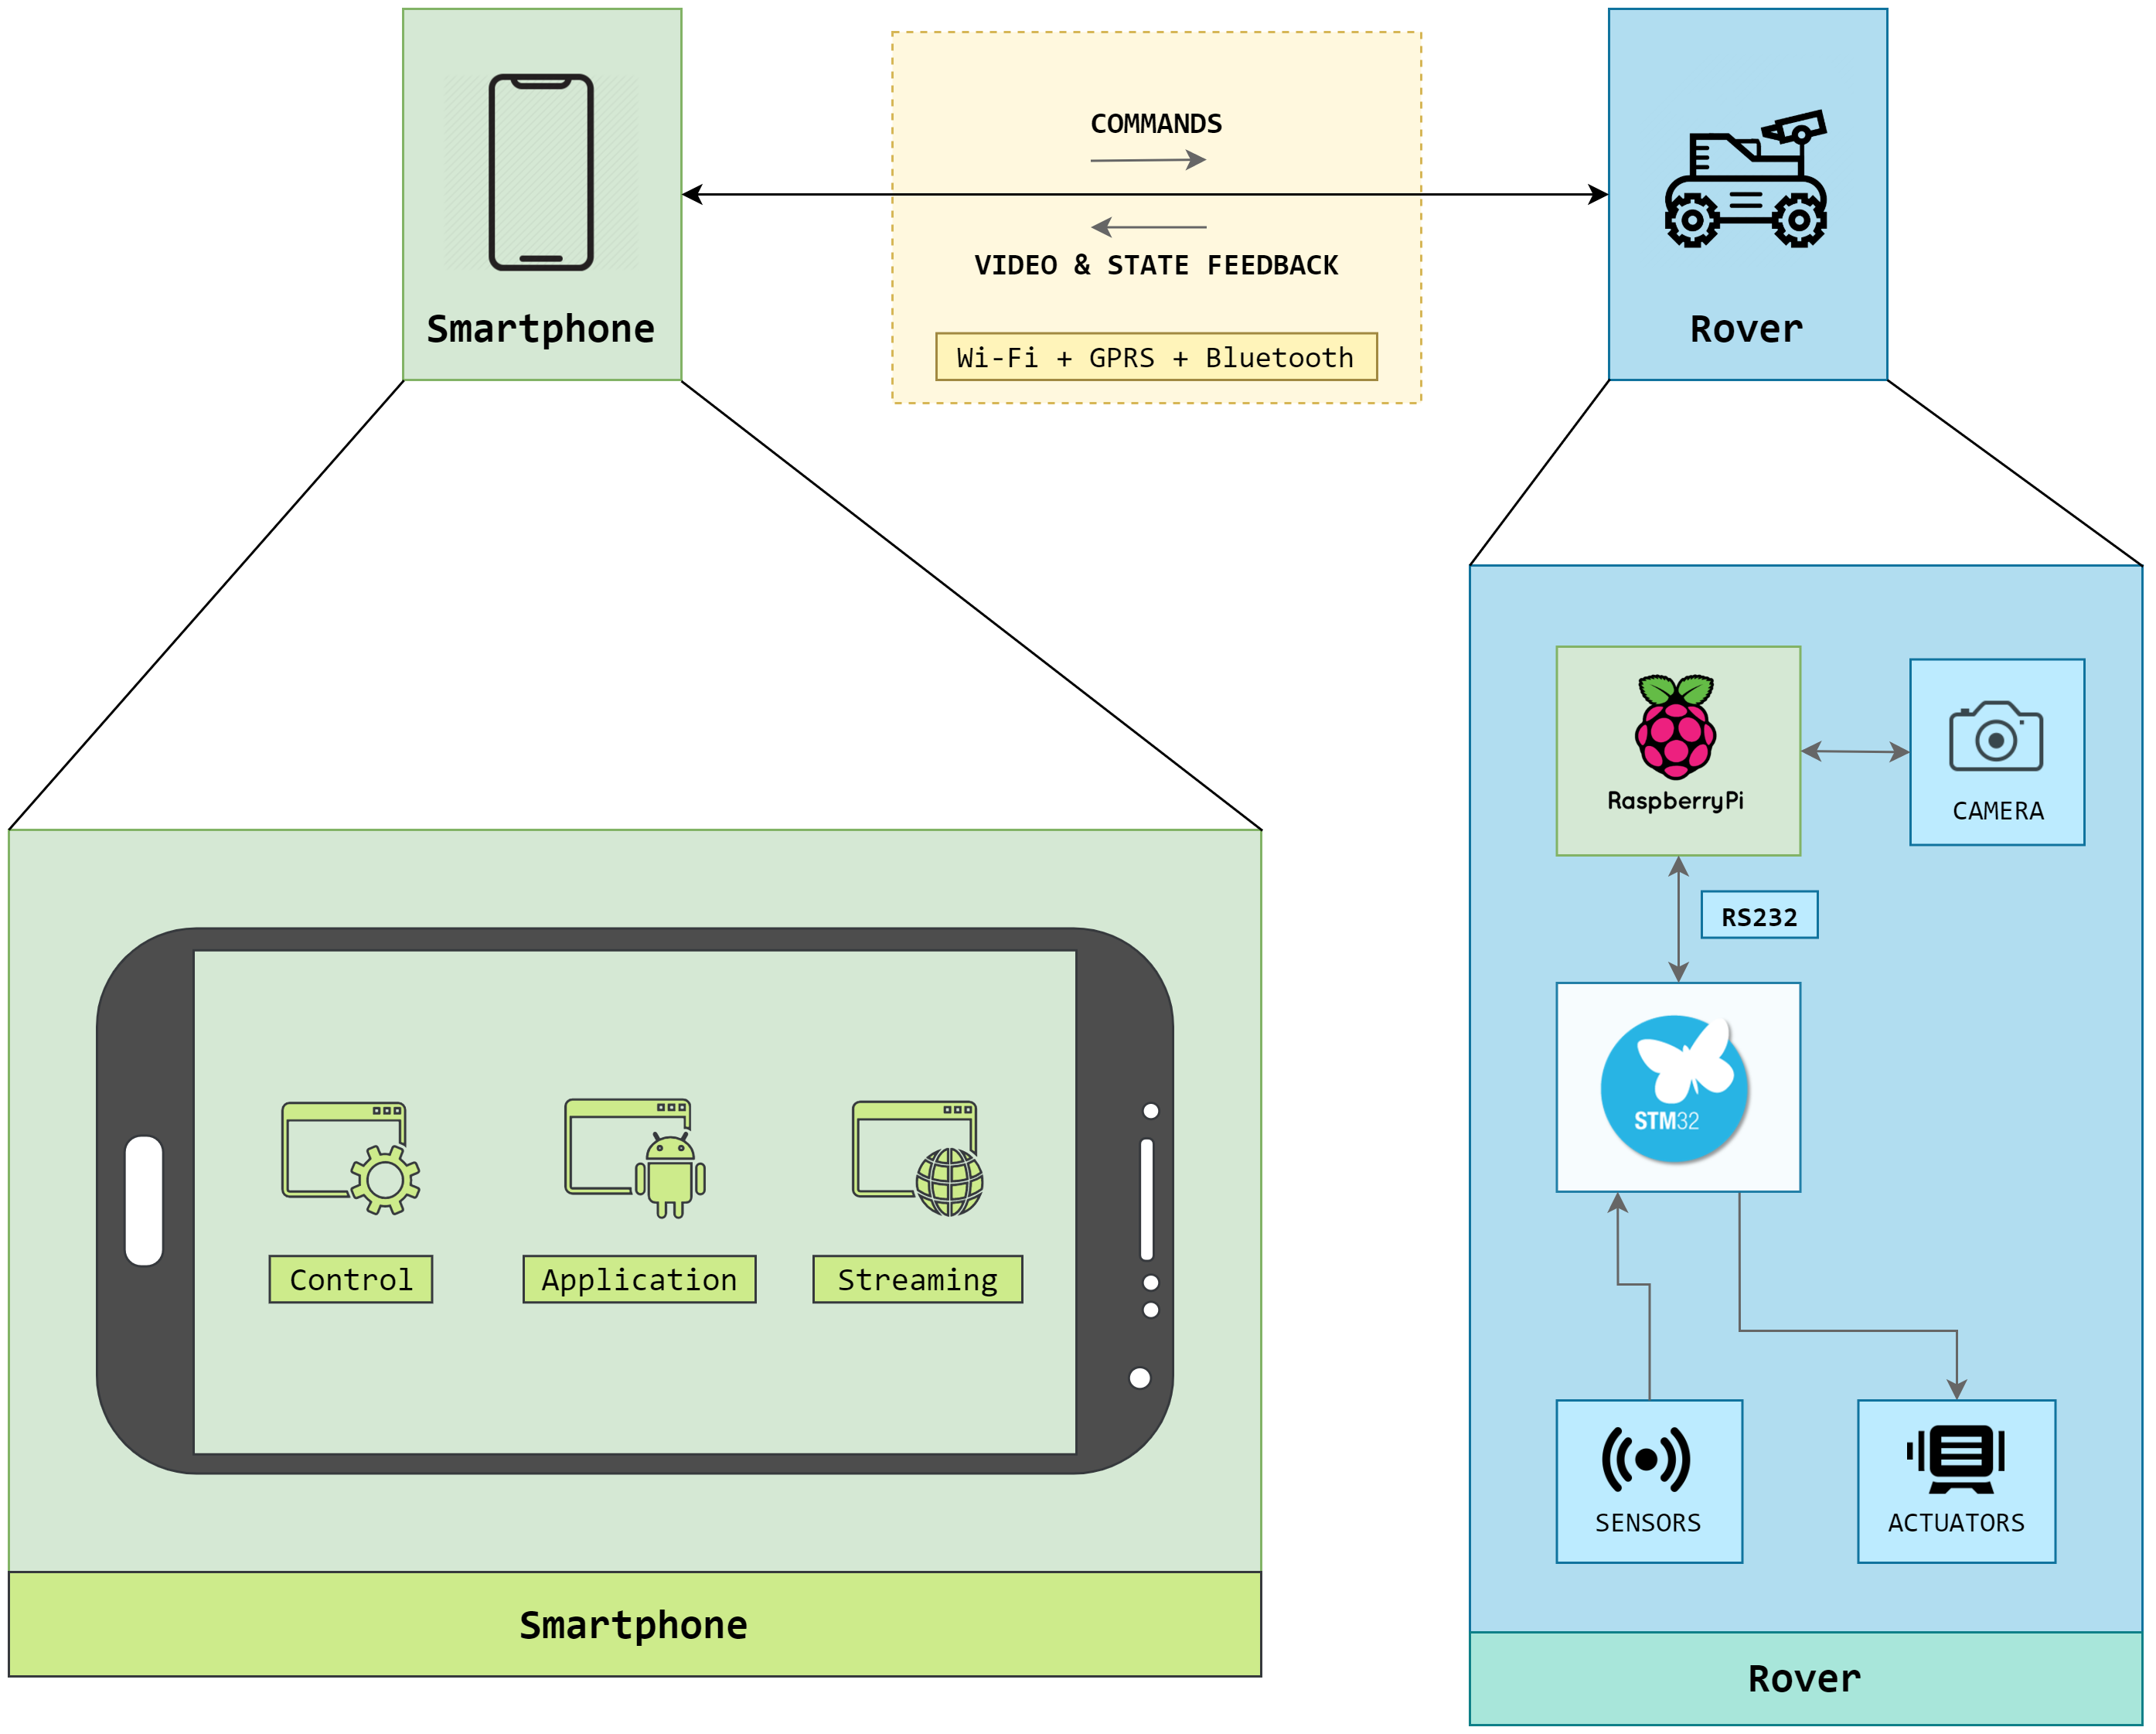
\includegraphics[width=1.0\textwidth]{./sec/img/initial_design_diagram.png}
\caption{\label{fig:initial-design}Initial design: Block diagram view}
\end{figure}

Thus, summarising, the initial design yields the system illustrated in
fig.~\ref{fig:initial-design}, comprised of:

\begin{itemize}
\item \textbf{ Raspberry Pi}: Interfaces with the camera directly, transmitting the information it receives to the smartphone. Receives user commands and sends sensorial information back to it;

\item \textbf{STM32}: Sends sensorial information to the Raspberry Pi module and receives commands from it. Controls the actuators according to the given instructions and sensor readings;

\item \textbf{Actuators}: DC Motors that control the car´s movement and headlights for nocturnal or low light conditions;

\item \textbf{Sensors}: Odometric sensors that support the detection of obstacles and luminosity sensors;

\item \textbf{Camera}: Device connected to the Raspberry Pi that allows the live stream of the car´s surrounding environment;

\item \textbf{Smartphone}: Grant visual feedback from the camera´s live feed also allowing the user to control the movement of the vehicle intuitively;

\end{itemize}

%%% Local Variables:
%%% mode: latex
%%% TeX-master: "../Phase1"
%%% End:
%
\section{Foreseen specifications tests}%
\label{sec:planning}
\section{Tests}%
\label{sec:org3e2776f}
Tests are generally considered as those performed over any physical
component or prototype. Here, however, it is used in a broader sense, to reflect the tests
conducted into the system and the several prototypes, under the abnormal present
circumstances. The tests are divided into verification and validation tests.
\subsection{Verifications tests}%
\label{sec:orge9c79e2}
The verifications tests are tests performed internally by the design team to
check the compliance of the foreseen specifications. These tests are done after
the prototype alpha is concluded.

\subsubsection{Functionality}%
\label{sec:functionality}
The remotely operated vehicle is composed of several modules distributed along
several different platforms, some of which distanced from each other. In the
present abnormal circumstances, this is even more true. Thus, the proposed sets
of functionalities should be tested in the integrated system, by tracking and
analysing the user commands issued along the way until it finally reaches the
vehicle, assessing if it is correctly processed. For example, if the user issues
the vehicle to move to a given place, the message sent to the vehicle must be
signaled in each endpoint hit, and the vehicle should move to that place.

\subsubsection{Maximum Load}%
\label{sec:load}
The remotely controlled vehicle can be used in applications involving load
carrying (besides its own, obviously), e.g., packet delivery. For this purpose
it is important to determine the maximum load the vehicle can carry safely at
the minimum velocity defined. As the load increases, also increases the power
consumption, diminishing the autonomy. Thus, two alternative definitions, and
consequently, tests arise for the maximum load determination:
\begin{enumerate}
\item maximum load (at minimum velocity): maximum load the vehicle can carry
  safely at the minimum velocity defined.
\item maximum load (at 50\% over the mean power consumption): maximum load which
  causes a 50\% increase in the mean power consumption, i.e., while operating at
  mean velocity.
\end{enumerate}

To test the former, load should be increased slowly, measuring the vehicle
mean velocity, until the minimum velocity defined is achieved. To test the
latter, load should be increased slowly, measuring the power consumption, until
a 50\% increase over the mean power power consumption is detected, while
operating at the mean velocity.

\subsubsection{Autonomy}%
\label{sec:org532616f}
The vehicle is operated off-the-grid, thus, a portable power source must be
included. The autonomy --- time interval between battery fully charged and
safely discharged --- should be observed for the following scenarios:
\begin{enumerate}
\item No load and vehicle operating at maximum speed
\item No load and vehicle operating at mean speed
\item Maximum load and vehicle operating at maximum speed
\item Maximum load and vehicle operating at mean speed
\end{enumerate}
The autonomy is related to product's power consumption and the capacity of the
battery chosen. Under the present abnormal circumstances is not reasonable to
expect the product's power consumption to match the real one, thus, for all
purposes, this will be considered as the one drawn by the car module itself,
namely, the installed motors and sensors.

Then, the autonomy can be measured as
the time interval between battery fully charged and safely discharged (the car
stops), by fixating the car to a supporting structure with free moving wheels,
and imposing the aforementioned conditions.

\subsubsection{Velocity}%
\label{sec:org20789b4}
The vehicle must be operated within a safe range of velocity, while also not
increasing excessively the power consumption. Thus, these velocity boundaries
should be tested in the absence of an external load and in the presence of the
maximum load. It is important to define these boundaries as follows:
\begin{itemize}
\item minimum velocity: minimum velocity defined for the vehicle, which must be
  attained even in the condition of maximum load. This value must be selected to
  assure safe motor operation.
\item maximum velocity (no load): maximum velocity for the vehicle in the
  absence of an external load. This is the absolute maximum velocity for the
  vehicle.
\item maximum velocity (maximum load): maximum velocity for the vehicle in the
  presence of the maximum load. This value must be selected to prevent excessive
  power consumption and motor overheating.
\end{itemize}
The aforementioned velocities should be tested in the designed conditions,
within a sufficiently long distance to assure velocity reach and stabilization,
and compared to the ones provided in the foreseen specifications.

\subsubsection{Safety}%
\label{sec:orgf4c025f}
Safety is paramount in product design, especially considering the vehicle is to
be remotely operated. Safety can be analysed in two ways, considering the
preservation of people and goods. For the former, it is important to assure safe
user operation as well as safe human interaction --- the vehicle may encounter
several people along its path, but it must not inflict any damage. For the
latter, the vehicle under operating conditions must not inflict any damage to
goods.

To test human safety, it is important to identify the interactions between the
user and the product, and which are the most prevalent and dangerous. Even so,
the exhaustive test is outside the scope of the present work; a small set of
features will be tested accordingly to the devised user manual, containing the
safety measures. For example, battery installation and conditions should be
tested, eventually leading to the posterior incorporation of safety measures in
the product.

To test goods safety, it is reasonable to assume the operating conditions of the
vehicle. Under these it is important to consider the most critical ones that
concern the moments when the vehicle is left to be controlled locally, instead
of user controlled operation. The critical conditions for local operations are
divided into two sets:
\begin{itemize}
\item processing of user commands and vehicle operation: user commands can
  conflict with safety measures and, thus, should be overriden locally.
\item communication loss: the vehicle is left to odometric navigation,
  preserving the safety of people and goods.
\end{itemize}
To test these two scenarios, they should be replicated, observing the system
response and tolerance.%DONE

\subsubsection{Image acquisition}%
\label{sec:orgb1f5c2a}
The vehicle is equipped with a camera to assist the user in its navigation,
thus, requiring it to be feed to the user's platform within proper conditions.
The following variables are to be tested: frame rate, range, and resolution.

\paragraph{Frame rate}%
\label{sec:frame-rate-test}
The frame rate is the rate at which the user platform screen is updated with new
image information. It should be maintained within acceptable boundaries to serve
the purpose of assisting the user in the vehicle's navigation. To test it, the
number of frame displayed per second in the user screen must be updated and
checked against the defined boundaries.

\paragraph{Range}%
\label{sec:range-test}
The range is the maximum distance the camera can clearly effectively capture an
image without losing resolution. To test this, an object must be captured at
increasing distances, until the image resolution is lost.

\paragraph{Resolution}%
\label{sec:resolution-test}
The image resolution quantifies how close lines can be to each other and still
be visibly resolved, giving an information on the its detail. The minimum
resolution should be tested as providing the least amount of information
required for the user, while minimizing data transfer and processing overhead.

\subsubsection{Communication reliability}%
\label{sec:comm-reli}
A communication is reliable if it guarantees measures to deliver the data
conveyed in the communication link. As reliability imposes these measures, it
also adds overhead to the communication protocol, which must be considered
depending on the case. For example, for the devised product, an user command
must be acknowledged to be processed, otherwise, the user must be informed; on
the other hand, loosing frames from the video feed is not so critical --- user
can still observe conveniently the field of vision if the frame rate is within
acceptable boundaries. 

Thus, given the critical nature of user commands issued, the focus will be on
this communication link. To test the reliability dummy packets should be sent
from the user platform to the vehicle and be acknowledged and parsed correctly.

\subsubsection{Closed loop error (Control loops)}%
\label{sec:closed-loop-error}
The velocity, direction and distance to obstacles must be continuosly monitored
to ensure proper vehicle operation. The closed loop error must then be checked
mainly in three situations as a response to an user command:
\begin{itemize}
\item velocity: the user issued an command with a given mean velocity, which
  should be compared with the steady-state mean velocity of the vehicle. This
  can be tested by comparing the user defined velocity and the vehicle's;
\item direction: the user issued an command with a given direction, which should
  be compared to the vehicle direction. This can be tested by measuring the
  angle between final and initial points and comparing it with the user defined
  direction.
\item distance to obstacles: the user issued an command with a given direction
  and velocity which can cause it to crash. The local control must take over
  control, preventing this to happen, and the final distance to the obstacles
  must be assessed and compared to the defined one.
\end{itemize}

%An overshoot occurs when the output in a control system exceeds its final,
%steady state value generally caused by a sudden change in the system, in this
%case specifically, the placement of a load upon the conveyor will cause an
%overshoot in the latter’s velocity which must be controlled lest it cause
%problems.
%
%An overshoot will occur during the settling time, as such, using the same
%considerations taken in its measurement, it can be measured by observing the
%induced voltage at the generator (an overshoot in the conveyor’s velocity will
%correspond to a peak in the generator’s voltage).
%
%Using an oscilloscope to display the induced voltage at the generator and making
%use of the “single mode” present in these measuring instruments one can observe
%the change that will occur in the generator’s induced voltage, the peak voltage
%that will be seen when the load is placed upon the running conveyor is the
%electrical representation of the overshoot of velocity, then either by
%converting it to its physical representation or comparing it to the reference
%voltage one can arrive at a conclusion. It was agreed that the overshoot
%velocity should be \(V_{ss} \pm 10\%\), where \(V_{ss}\) is the stedy state
%velocity.

\subsection{Validation tests}%
\label{sec:orgff1a37d}
The validation tests should be performed by the client using the product’s
manual, so it is expected that a user without prior experience with the product
should be able to use it correctly and safely. On the present abnormal
circumstances, with limited access to the physical modules, specially for an
external agent, the validation is severely limited.
Thus, it should be limited to user interface validation.

For this purpose, an external agent will be provided with the software
application and the respective installation and usage manuals, and the feedback
will be collected and processed to further improve the product.
%%% Local Variables:
%%% mode: latex
%%% TeX-master: "../Phase1"
%%% End:

%
%%% Local Variables:
%%% mode: latex
%%% TeX-master: "../../../dissertation"
%%% End:
  \setcounter{table}{0}
  \setcounter{figure}{0}
  %
  \chapter{Design}%
\label{ch:design}
The envisioned product consists of a remote controlled car used to assist
exploration and maintenance domains, hereby, denominated as Radio Frequency
Camera Assisted Rover (RFCAR). To satisfy such requirements, the vehicle must
contain a remotely operated camera that provides a live video feed to the user.
Additionally, the vehicle must include an odometric system that assists the
driving and avoids unintentional collisions when remote control is compromised, e.g., when connection is lost.
The vehicle provides means for exploration and conditions assessment in critical
or unaccessible areas to human operators, such as fluid pipelines and other hazardous locations.
%
%%% Local Variables:
%%% mode: latex
%%% TeX-master: "../Report"
%%% End:

  \setcounter{table}{0}
  \setcounter{figure}{0}
  %%\begin{document}
% CHAPTER - Contribution -------------------------
\chapter{Development}
\label{ch:development}
%
In this chapter, the knowledge acquired through the relevant models contained

The implementation of this thread is presented
in listing~\ref{lst:threadSerialRx}.
%
% LISTING: ThreadSerialRx
\lstinputlisting[language=C++, caption={Thread Serial Rx handler},label=lst:threadSerialRx,
style=customc]{./listing/threadSerialRx.cpp}%

%


%
%%% Local Variables:
%%% mode: latex
%%% TeX-master: "../../../dissertation"
%%% End:

  % CHAPTER - Implementation ---------------
\chapter{Implementation}%
\label{ch:implementation}
  The multi-material part fabrication is a complex topic and most current
  commercially available systems have been designed for mono-material part
  fabrication~\cite{wohlers2011wohlers} and are unprepared for multi-material
  processing due to the lack of flexibility and processing capability.
%
\section{Navigation Virtual Subsystem}%
\label{sec:navig-virt-subsyst-implem}
%\input{./tex/Chap/Implem/navig}
%
\subsection{Control}%
\label{sec:control-design}
%\input{./tex/Chap/Implem/navig}
%
\section{Physical Environment Virtual Subsystem}%
\label{sec:phys-envir-virt-design}
%\input{./tex/Chap/Implem/navig}
%
\section{Remote Vision Virtual Subsystem}%
\label{sec:remote-visi-subsyst-design}
%\input{./tex/Chap/Implem/navig}
%
\section{Smartphone}%
\label{sec:smartphone-design}
% \input{./tex/Chap/Implem/navig}
%
%%% Local Variables:
%%% mode: latex
%%% TeX-master: "../../../dissertation"
%%% End:

  \setcounter{table}{0}
  \setcounter{figure}{0}
  %
  %% CHAPTER - Application -------------------------
\chapter{Tests}
\label{ch:application}
In this chapter, the \gls{lbam} methodology devised was tested and the results

% Please add the following required packages to your document preamble:
% \usepackage{multirow}
\begin{table}[!hbt]
\centering
\caption{\gls{mms} machine final specifications}
\label{tab:mach-final-specs}
\begin{tabular}{ll}
\hline
Dimensions (l x w x h){[}mm{]} & 560 x 450 x 280 \\ \hline
\multirow{2}{*}{Power supply} & Laser: 400 VAC, 10 A \\ \cline{2-2} 
 & Machine: 24 V, 15 A \\ \hline
Build dimensions {[}mm{]} & 50 x 50 x 50 \\ \hline
Nr. of materials & 2 \\ \hline
Temperature & Tested up to 250$^{\circ}$C (higher temperatures can be used) \\ \hline
\multirow{3}{*}{Laser} & Type: $CO_2$ \\ \cline{2-2} 
 & Power: 30 W \\ \cline{2-2} 
 & Spot size: 50 $\mu$m \\ \hline
  \multirow{2}{*}{Resolution {[}$\mu$m{]}} & Full-step (all axes, except bed): 5 $\pm$ 0.25 \\ \cline{2-2} 
 & 1/16-step (bed): 0.32 $\pm$ 0.016 \\ \hline
\multirow{3}{*}{Estimated cost {[}EURO{]}} & Laser: 7500 \\ \cline{2-2} 
 & Machine: 1500 \\ \cline{2-2} 
 & Total: 9000 \\ \hline
\end{tabular}
\end{table}

\section{Summary}
In this chapter tests were performed on the workflow, equipment and
%%% Local Variables:
%%% mode: latex
%%% TeX-master: "../../../dissertation"
%%% End:

  \chapter{Testing}%
\label{ch:implem}
The envisioned product consists of a remote controlled car used to assist
exploration and maintenance domains, hereby, denominated as Radio Frequency
Camera Assisted Rover (RFCAR). To satisfy such requirements, the vehicle must
contain a remotely operated camera that provides a live video feed to the user.
Additionally, the vehicle must include an odometric system that assists the
driving and avoids unintentional collisions when remote control is compromised, e.g., when connection is lost.
The vehicle provides means for exploration and conditions assessment in critical
or unaccessible areas to human operators, such as fluid pipelines and other
hazardous locations.
%
%%% Local Variables:
%%% mode: latex
%%% TeX-master: "../Report"
%%% End:
  \setcounter{table}{0}
  \setcounter{figure}{0}
  %
  %% CHAPTER - Application -------------------------
\chapter{Tests}
\label{ch:application}
In this chapter, the \gls{lbam} methodology devised was tested and the results

% Please add the following required packages to your document preamble:
% \usepackage{multirow}
\begin{table}[!hbt]
\centering
\caption{\gls{mms} machine final specifications}
\label{tab:mach-final-specs}
\begin{tabular}{ll}
\hline
Dimensions (l x w x h){[}mm{]} & 560 x 450 x 280 \\ \hline
\multirow{2}{*}{Power supply} & Laser: 400 VAC, 10 A \\ \cline{2-2} 
 & Machine: 24 V, 15 A \\ \hline
Build dimensions {[}mm{]} & 50 x 50 x 50 \\ \hline
Nr. of materials & 2 \\ \hline
Temperature & Tested up to 250$^{\circ}$C (higher temperatures can be used) \\ \hline
\multirow{3}{*}{Laser} & Type: $CO_2$ \\ \cline{2-2} 
 & Power: 30 W \\ \cline{2-2} 
 & Spot size: 50 $\mu$m \\ \hline
  \multirow{2}{*}{Resolution {[}$\mu$m{]}} & Full-step (all axes, except bed): 5 $\pm$ 0.25 \\ \cline{2-2} 
 & 1/16-step (bed): 0.32 $\pm$ 0.016 \\ \hline
\multirow{3}{*}{Estimated cost {[}EURO{]}} & Laser: 7500 \\ \cline{2-2} 
 & Machine: 1500 \\ \cline{2-2} 
 & Total: 9000 \\ \hline
\end{tabular}
\end{table}

\section{Summary}
In this chapter tests were performed on the workflow, equipment and
%%% Local Variables:
%%% mode: latex
%%% TeX-master: "../../../dissertation"
%%% End:

  % CHAPTER - Verification and Validation ---------------
\chapter{Verification and Validation}%
\label{ch:Validation}
  The multi-material part fabrication is a complex topic and most current
  commercially available systems have been designed for mono-material part
  fabrication~\cite{wohlers2011wohlers} and are unprepared for multi-material
  processing due to the lack of flexibility and processing capability.
  %
%
\section{Verification}%
\label{sec:verification}
% \input{./tex/Chap/Verif-Valid/verification}
%
\section{Validation}%
\label{sec:validation}
% \input{./tex/Chap/Verif-Valid/validation}
%
%
%%% Local Variables:
%%% mode: latex
%%% TeX-master: "../../../dissertation"
%%% End:

  \setcounter{table}{0}
  \setcounter{figure}{0}
  %
  	% CHAPTER - Conclusion/Future Work --------------
\chapter{Conclusion}
\label{ch:conclusion}
In this chapter the conclusions and prospect for future work are presented.

%%% Local Variables:
%%% mode: latex
%%% TeX-master: "../../../dissertation"
%%% End:

  \setcounter{table}{0}
  \setcounter{figure}{0}
  % -----------------------------------------------------------------
  %
	\bookmarksetup{startatroot} % Ends last part.
	%\addtocontents{toc}{\bigskip} % Making the table of contents look good.
	%\cleardoublepage
%
	%- Bibliography (needs bibtex) -%
  % Using relative paths: 
  % src: https://tex.stackexchange.com/questions/38287/creating-a-central-bibliography
  %\addcontentsline{toc}{chapter}{Bibliography}
  \bibliography{./bib/dissert}
%
  % bibliography - tutorial: 
  % https://en.wikibooks.org/wiki/LaTeX/Modular_Documents
  %\clearpage %see what this means
  %\include{./tex/mybibliography}
%
  % ---------------------- APPENDIX ------------------------------------
  % renew figures and tables to use Alphabetic numbering and set counter to zero
  % src: https://tex.stackexchange.com/questions/118606/numbering-tables-a1-a2-etc-in-latex#comment862599_311998
  \setcounter{table}{0}
  \setcounter{figure}{0}
  \renewcommand{\thetable}{\Alph{chapter}.\arabic{table}}  
  \renewcommand{\thefigure}{\Alph{chapter}.\arabic{figure}}
 %
  % Adding a page to separate appendices from the other chapters
  \chapter*{Appendices}%
\label{ch:Append}
  \addcontentsline{toc}{chapter}{\normalfont\scshape{Appendices}}
  \cleardoublepage%
%
  %\appendix % this is the normal appendix; we use a custom one
  \umappendix{Appendix}
%
  % Appendix chapters inclusion
  %
\setcounter{table}{0}
\setcounter{figure}{0}
% the appendix no longer requires the prefix Appendix <Letter>
\chapter{Use cases (Detailed description)}%
\label{ch:append-UseCases}
In this section, the main use cases are described extensively. As many uses
cases are similar, only changing the parameter to which they refer to, the
Lighting subsystem was used as an example for the Manage<Parameter> use case,
where <Parameter> is Temperature, DoorBell, DateAndTime and SystemNotifications.

\begin{table}
  \captionsetup{justification=raggedright, singlelinecheck=false}
  \caption{Use case LoadGeometryFile}
  \centering
  \begin{tabular}{p{0.26\textwidth}p{0.64\textwidth}}
    \hline
    Use case name & \textbf{LoadGeometryFile} \\ \hline
     Participating actors      & Initiated by the User \\ \hline
     Flow of events & \begin{enum-c}
     \item The User selects the load geometry file option.
     \item The User selects the geometry file to load from a list.
     \item If the file is successfully loaded, the filename is displayed,
       and the file previewed (include \underline{PreviewGeometryFile} use
       case).
     \item Otherwise, an error message is displayed to the user.
     \end{enum-c}\\ \hline 
     Entry conditions       & The User has started the MMSLS machine control
     software and has previously generated a valid geometry file. \\ \hline 
      Exit conditions & The file is successfully loaded, previewed and with the
      filename displayed or an error message is displayed to the User.\\ \hline 
      Quality requirements &  Feedback must be given to the user within 2
      seconds; if files are ``heavy'', display an ongoing processing.\\ \hline 
  \end{tabular}
\label{tab:us-load-geom}
\end{table}

\begin{table}
  \captionsetup{justification=raggedright, singlelinecheck=false}
  \caption{Use case PreviewGeometryFile}
  \centering
  \begin{tabular}{p{0.26\textwidth}p{0.64\textwidth}}
    \hline
    Use case name & \textbf{PreviewGeometryFile} \\ \hline
     Participating actors      & Initiated by the User \\ \hline
     Flow of events & \begin{enum-c}
     \item The User loads the geometry file.
     \item The geometry file is displayed on the canvas.
     \end{enum-c}\\ \hline 
     Entry conditions       & A valid geometry file is loaded into the
     application. \\ \hline 
      Exit conditions & The geometry file is displayed on canvas.      \\ \hline 
      Quality requirements & The preview should be resizable to accommodate
      the various component's dimensions. \\ \hline 
  \end{tabular}
\label{tab:us-prev-geom}
\end{table}

\begin{table}
  \captionsetup{justification=raggedright, singlelinecheck=false}
  \caption{Use case AssignColorsToLaserParams}
  \centering
  \begin{tabular}{p{0.26\textwidth}p{0.64\textwidth}}
    \hline
    Use case name & \textbf{AssignColorsToLaserParams} \\ \hline
     Participating actors      & Initiated by the User \\ \hline
     Flow of events & \begin{enum-c}
     \item The User selects a layer.
     \item The User associates a material's color to its laser's processing color
       counterpart.
     \item The User can edit the laser's processing color attributes.
     \end{enum-c}\\ \hline 
     Entry conditions       & The file is successfully loaded into the
     application and the preview is editable. \\ \hline 
      Exit conditions & The materials' colors has been assigned to valid laser's
      processing color with the respective processing parameters.\\ \hline 
      Quality requirements & Allow multiple line selection. \\ \hline 
  \end{tabular}
\label{tab:us-assign-colors}
\end{table}

\begin{table}
  \captionsetup{justification=raggedright, singlelinecheck=false}
  \caption{Use case LoadManufFile}
  \centering
  \begin{tabular}{p{0.26\textwidth}p{0.64\textwidth}}
    \hline
    Use case name & \textbf{LoadManufFile} \\ \hline
     Participating actors      & Initiated by the User \\ \hline
     Flow of events & \begin{enum-c}
     \item The User selects the load manufacturing file option.
     \item The User selects the manufacturing file to load from a list.
     \item If the file is successfully loaded, the filename is displayed.
     \item Otherwise, an error message is displayed to The User.
     \end{enum-c}\\ \hline 
     Entry conditions       & The User has started the MMSLS machine control
     software and has previously generated a valid manufacturing file. \\ \hline 
      Exit conditions & The file is successfully loaded and with the
      filename displayed or an error message is displayed to the User.      \\ \hline 
      Quality requirements & Feedback must be given to the user within 2
      seconds; if files are 'heavy', display an ongoing processing. \\ \hline 
  \end{tabular}
\label{tab:us-load-manuf}
\end{table}

\begin{table}
  \captionsetup{justification=raggedright, singlelinecheck=false}
  \caption{Use case ConnectToMach}
  \centering
  \begin{tabular}{p{0.26\textwidth}p{0.64\textwidth}}
    \hline
    Use case name & \textbf{ConnectToMach} \\ \hline
     Participating actors      & Initiated by the User \\ \hline
     Flow of events & \begin{enum-c}
     \item The User selects the appropriate connection to the machine from a list.
     \item The User selects the \emph{Connect to Machine} option.
     \item If the connection is successful, the connection status is updated to
       \emph{Connected} and machine operation options are enabled.
     \item Otherwise, an error message is displayed to The User.
     \end{enum-c}\\ \hline 
     Entry conditions       & The User has started the MMSLS machine control
     software and there is physical connection between the \emph{Master} system and
     the \gls{mms}  machine. \\ \hline 
      Exit conditions & The connection is established between \emph{Master} system and
      the \gls{mms} machine or an error message is displayed to the user.\\ \hline 
  \end{tabular}
\label{tab:us-con-to-mach}
\end{table}

\begin{table}
  \captionsetup{justification=raggedright, singlelinecheck=false}
  \caption{Use case DisconnectToMach}
  \centering
  \begin{tabular}{p{0.26\textwidth}p{0.64\textwidth}}
    \hline
    Use case name & \textbf{DisconnectToMach} \\ \hline
     Participating actors      & Initiated by the User \\ \hline
     Flow of events & \begin{enum-c}
     \item The User selects the \emph{Disconnect to Machine} option.
     \item If the disconnection is successful, the connection status is updated to
       \emph{Disconnected} and machine operation options are disabled.
     \item Otherwise, an error message is displayed to The User.
     \end{enum-c}\\ \hline 
     Entry conditions       & A successful connection between the \emph{Master} system
     and the \gls{mms} machine is established.\\ \hline 
      Exit conditions & The connection is closed and the machine operations
      options are disabled or an error messaged is displayed to the user \\ \hline 
  \end{tabular}
\label{tab:us-discon-to-mach}
\end{table}

\begin{table}
  \captionsetup{justification=raggedright, singlelinecheck=false}
  \caption{Use case ManualResetMach}
  \centering
  \begin{tabular}{p{0.26\textwidth}p{0.64\textwidth}}
    \hline
    Use case name & \textbf{ManualResetMach} \\ \hline
     Participating actors      & Initiated by the User \\ \hline
     Flow of events & \begin{enum-c}
     \item The User selects the axis to reset, the direction and the reset
       distance.
     \item When the reset is satisfactory, The User acknowledges this fact by
       selecting the option \emph{Reset end}.
     \item The option to \emph{Start Manufacturing} is now enabled.
     \end{enum-c}\\ \hline 
     Entry conditions       &  A successful connection between the \emph{Master}
     system and the \gls{mms} machine is established.\\ \hline 
      Exit conditions & The reset is satisfactory (User has selected option
      \emph{Reset End}) and the \emph{Start Manufacturing} is enabled.      \\ \hline 
      Quality requirements & Provide feedback to the User of the manual reset
      operations (ascent/descent of the axis) \\ \hline 
  \end{tabular}
\label{tab:us-man-reset}
\end{table}

\begin{table}
  \captionsetup{justification=raggedright, singlelinecheck=false}
  \caption{Use case StartManuf}
  \centering
  \begin{tabular}{p{0.26\textwidth}p{0.64\textwidth}}
    \hline
    Use case name & \textbf{StartManuf} \\ \hline
     Participating actors      & Initiated by the user \\ \hline
     Flow of events & \begin{enum-c}
     \item The User selects the \emph{Start manufacturing} option.
     \item If successful, the machine initiates the manufacturing process
       the machine status is updated to \emph{Run}.
     \end{enum-c}\\ \hline 
     Entry conditions       & \begin{enum-c}
     \item A successful connection between the \emph{Master} system
     and the \gls{mms} machine is established. 
      \item Reset is finished.
      \item Valid geometry and manufacturing file have been loaded.
     \end{enum-c}\\ \hline 
      Exit conditions & \begin{item-c}
      \item \emph{Success}: The \gls{mms} machine status is updated to \emph{Run}, the
        \emph{Start manufacturing} option is disabled, and the options
       \emph{Pause manufacturing} and \emph{Stop manufacturing} are enabled.
     \item \emph{Fail}: An error message is displayed to the user.
      \end{item-c}\\ \hline
      Quality requirements & Update the relevant processing information to the
        User (include use case \underline{UpdateInfo}). \\ \hline 
  \end{tabular}
\label{tab:us-start-manuf}
\end{table}

\begin{table}
  \captionsetup{justification=raggedright, singlelinecheck=false}
  \caption{Use case PauseManuf}
  \centering
  \begin{tabular}{p{0.26\textwidth}p{0.64\textwidth}}
    \hline
    Use case name & \textbf{PauseManuf} \\ \hline
     Participating actors      & Initiated by the user \\ \hline
     Flow of events & \begin{enum-c}
     \item The User selects the \emph{Pause manufacturing} option.
     \item If successful, the manufacturing process is paused.
     \end{enum-c}\\ \hline 
     Entry conditions       & The manufacturing has started (startManuf was
     triggered), but has not yet finished. \\ \hline 
      Exit conditions & \begin{item-c}
      \item \emph{Success}: The manufacturing process is paused, and
        the \gls{mms} machine status is updated to \emph{Idle}. The \emph{Pause
        manufacturing} option is disabled and the \emph{Start manufacturing}
        option is re-enabled.
     \item \emph{Fail}: An error message is displayed to the user.
      \end{item-c}\\ \hline
  \end{tabular}
\label{tab:us-pause-manuf}
\end{table}

\begin{table}
  \captionsetup{justification=raggedright, singlelinecheck=false}
  \caption{Use case StopManuf}
  \centering
  \begin{tabular}{p{0.26\textwidth}p{0.64\textwidth}}
    \hline
    Use case name & \textbf{StopManuf} \\ \hline
     Participating actors      & Initiated by the User \\ \hline
     Flow of events & \begin{enum-c}
     \item The User selects the \emph{Stop manufacturing} option.
     \item If successful, the manufacturing process is stopped.
     \end{enum-c}\\ \hline 
     Entry conditions & The manufacturing has started (startManuf was
     triggered), but has not yet finished. \\ \hline 
      Exit conditions & \begin{item-c}
      \item \emph{Success}: The manufacturing process is stopped, and
        the \gls{mms} machine status is updated to \emph{Stopped}. The
        \emph{Stop manufacturing} option is disabled and the \emph{Start
        manufacturing} option is re-enabled.
     \item \emph{Fail}: An error message is displayed to the user.
      \end{item-c}\\ \hline
  \end{tabular}
\label{tab:us-stop-manuf}
\end{table}

Although several notifications from relevant events are to be notified by the
\emph{Master} machine to the User, for brevity purposes only the most relevant one is
showcased here, namely \underline{NotifyManufEnd}.

\begin{table}
  \captionsetup{justification=raggedright, singlelinecheck=false}
  \caption{Use case NotifyManufEnd}
  \centering
  \begin{tabular}{p{0.26\textwidth}p{0.64\textwidth}}
    \hline
    Use case name & \textbf{NotifyManufEnd} \\ \hline
     Participating actors      & Initiated by MMS-Mach; User participates \\ \hline
     Flow of events & \begin{enum-c}
     \item When manufacturing is completed, the \emph{Master} system notifies The User
       about this fact.
     \end{enum-c}\\ \hline 
     Entry conditions & The manufacturing has started (startManuf was
     triggered), and is not paused or stopped. \\ \hline 
     Exit conditions & The manufacturing process stops and the User is notified
      about this fact.\\ \hline 
  \end{tabular}
\label{tab:us-notif-manuf-end}
\end{table}

\begin{table}[!hbt]
  \captionsetup{justification=raggedright, singlelinecheck=false}
  \caption{Use case VisualizeManuf}
  \centering
  \begin{tabular}{p{0.26\textwidth}p{0.64\textwidth}}
    \hline
    Use case name & \textbf{VisualizeManuf} \\ \hline
     Participating actors      & Initiated by MMS-Mach or Laser; User participates \\ \hline
     Flow of events & \begin{enum-c}
     \item Relevant manufacturing information is sent by the MMS-Mach or the
       Laser to the \emph{Master} system --- on a time-basis or triggered by a
       relevant event like the manufacturing completion of one layer --- that is
       updated to the User.
     \end{enum-c}\\ \hline 
     Entry conditions & The manufacturing has started (startManuf was
     triggered)\\ \hline
      Exit conditions & The manufacturing is stopped or has ended. \\ \hline 
      Quality requirements & \begin{item-c}
      \item \emph{Time-basis} The relevant manufacturing information must be
        updated with 1 second refresh rate.
      \item \emph{Event} The information associated with the triggering event
        must be updated immediately.
      \end{item-c} \\ \hline 
  \end{tabular}
\label{tab:vis-manuf}
\end{table}

%%% Local Variables:
%%% mode: latex
%%% TeX-master: "../../dissertation"
%%% End:

\setcounter{table}{0}
\setcounter{figure}{0}
%
\chapter{Sequence Diagrams}
\label{ch:append-seq-diag}
\begin{figure*}
  \begin{center}
    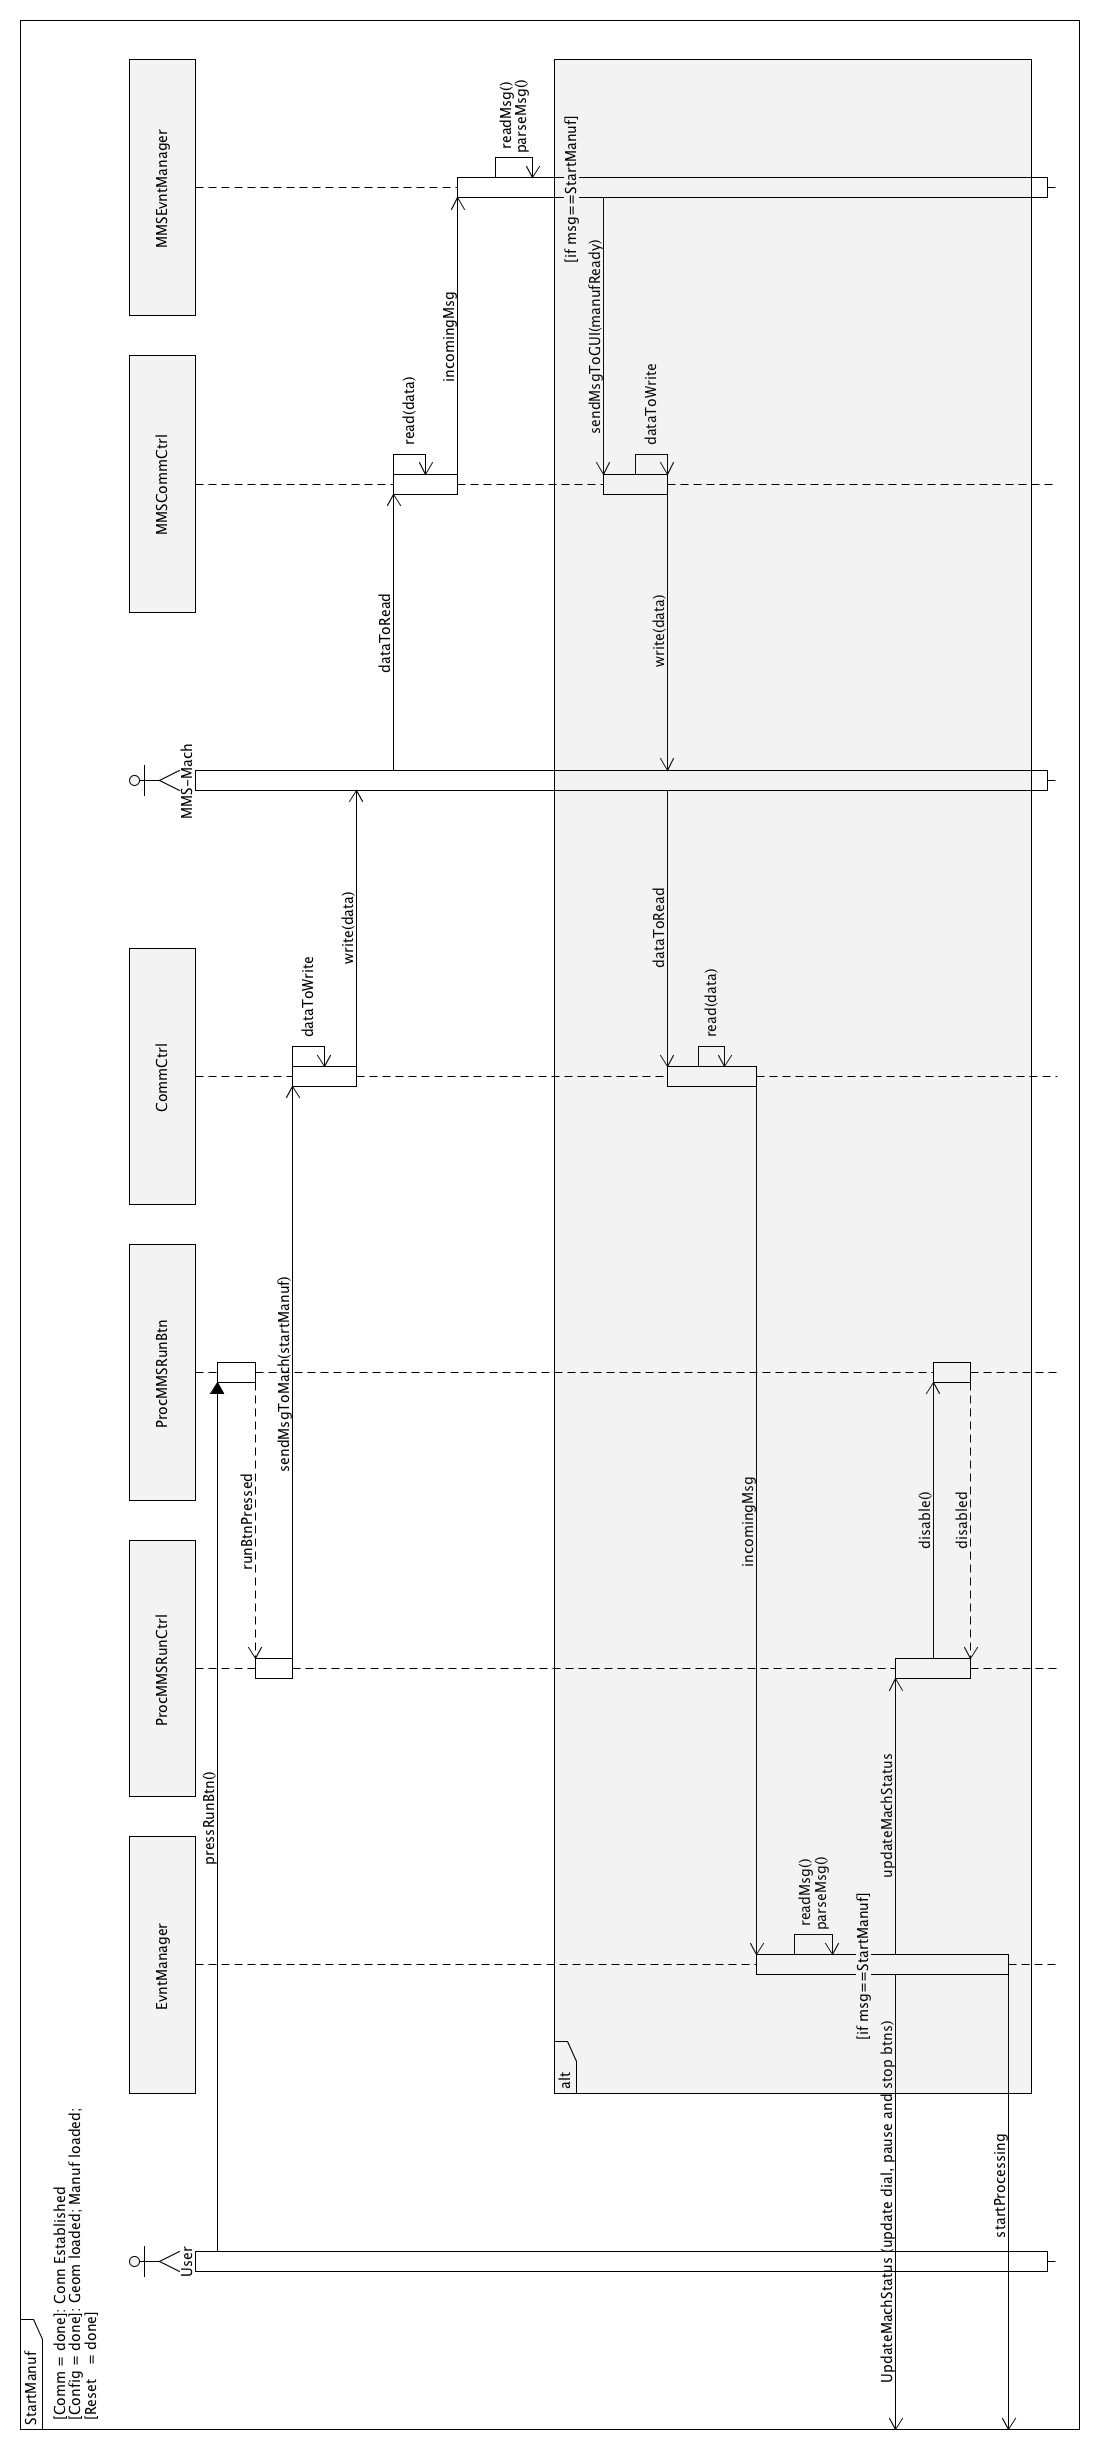
\includegraphics[height=1.0\textheight]{./img/seq-start-manuf-lscape.png}
  \end{center}
  \caption{Sequence diagram for the \emph{StartManuf} use case (Part 1)}\label{fig:seq-start-manuf-lscape}
\end{figure*}

\begin{figure*}
  \begin{center}
    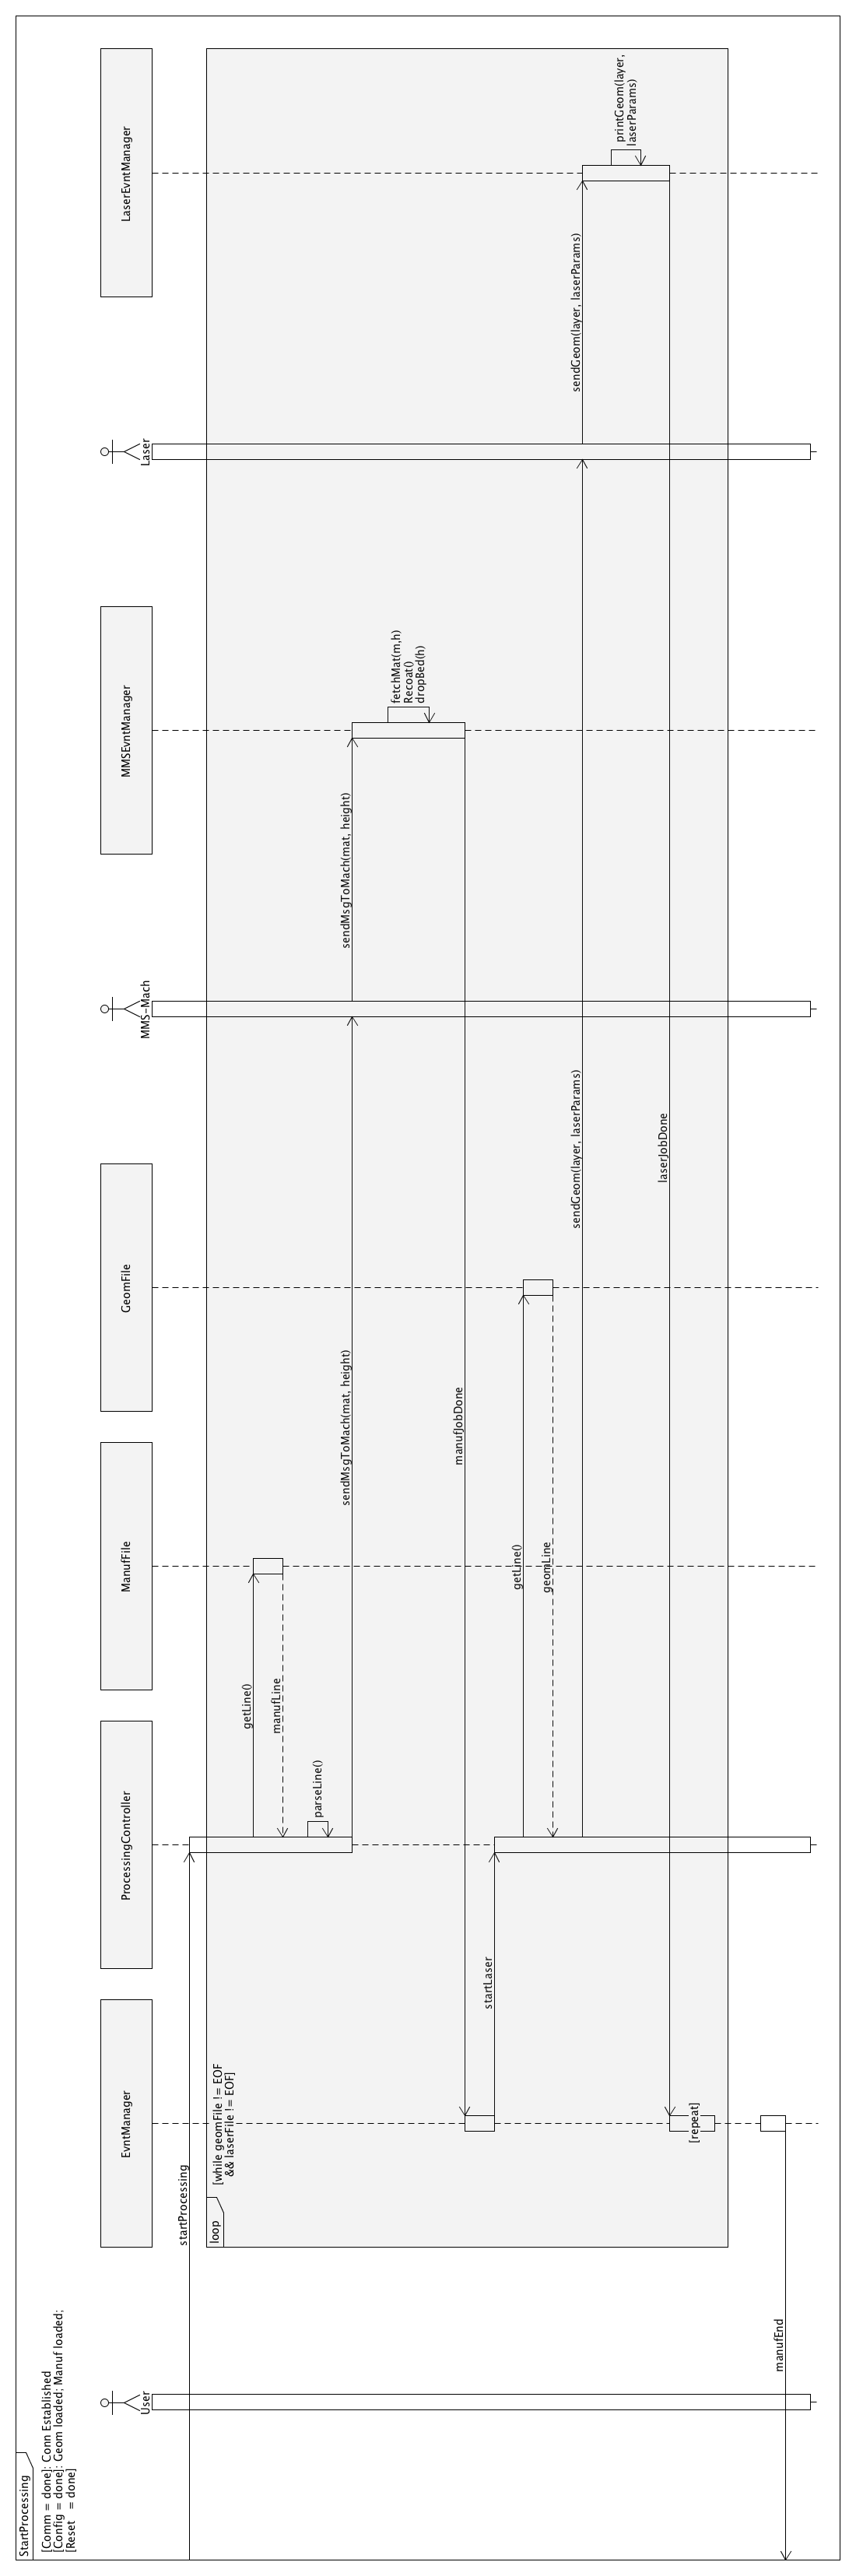
\includegraphics[height=1.0\textheight]{./img/seq-start-process-lscape.png}
  \end{center}
  \caption{Sequence diagram for the \emph{StartManuf} use case (Part 2)}\label{fig:seq-start-process-lscape}
\end{figure*}
%
%\clearpage
%
%% src:https://www.reddit.com/r/LaTeX/comments/4jynr7/adding_a3_pdf_page_into_an_a4_document/d3ba7eg/ 
%\KOMAoptions{paper=A3,pagesize}
%%\KOMAoptions{paper=landscape, pagesize}
%
%\label{ch:append-UseCases}
%\begin{figure*}
%  \begin{center}
%    \includegraphics[width=1.6\textwidth]{./img/seq-start-manuf.png}
%  \end{center}
%  \caption{Sequence diagram for the \emph{StartManuf} use case (Part 1)}%
%\label{fig:seq-start-manufA3}
%\end{figure*}
%
%\begin{figure*}
%  \begin{center}
%    \includegraphics[width=1.6\textwidth]{./img/seq-start-process.png}
%  \end{center}
%  \caption{Sequence diagram for the \emph{StartManuf} use case (Part 2)}%
%\label{fig:seq-start-processA3}
%\end{figure*}
%
%\cleardoublepage
%\KOMAoptions{paper=A4, pagesize}


%
	%\chapter{Support material}
	%Auxiliary results which are not main-stream; or
%
	%\chapter{Details of results}
	%Details of results whose length would compromise readability of main text; or
%
	%\chapter{Listings}
	%Specifications and Code Listings: should this be the case; or
%
	%\chapter{Tooling}
	%Tooling: Should this be the case.
%
	%Anyone using \Latex\ should consider having a look at \TUG,
	%the \tug{\TeX\ Users Group}
%
	% Back Cover -------------------------------------------
%	\umbackcover{
%%	NB: place here information about funding, FCT project, etc in which the
%%	work is framed. Leave empty otherwise.
%         % The author gratefully acknowledges the financial support of ``Fundação
%         % para a Ciência e Tecnologia'' (FCT – Portugal), through the research
%         % project PTDC/ECM/108146/2008 (“Generalised Beam Theory (GBT) –
%         % Development, Application and Dissemination”).
%         % HAMaBICo --- Hybrid Additive Manufacturing for Bio Inspired Component
%         % through the research project  NORTE-01-0145-FEDER-000018.
%          The author gratefully acknowledges the financial support of this
%          project through the research projects NORTE-01-0145-FEDER-000018
%          (HAMaBICo --- Hybrid Additive Manufacturing for Bio Inspired
%          Component) and POCI-01-0145-FEDER-030498 (FunImp --- Design and
%          Fabrication of MultiFunctional Implants).
%	}
\end{document}
%%% Local Variables:
%%% mode: latex
%%% TeX-master: t
%%% End:
